
\let\negmedspace\undefined
\let\negthickspace\undefined
\documentclass[journal,12pt,twocolumn]{IEEEtran}
%\documentclass[conference]{IEEEtran}
%\IEEEoverridecommandlockouts
% The preceding line is only needed to identify funding in the first footnote. If that is unneeded, please comment it out.
\usepackage{cite}
\usepackage{amssymb,amsfonts,amsthm,amsmath}
\usepackage{algorithmic}
\usepackage{graphicx}
\usepackage{textcomp}
\usepackage{xcolor}
\usepackage{txfonts}
\usepackage{listings}
\usepackage{enumitem}
\usepackage{mathtools}
\usepackage{gensymb}

%%
%\usepackage{setspace}
%%\doublespacing
%\singlespacing
%
%%\usepackage{graphicx}
%%\usepackage{amssymb}
%%\usepackage{relsize}
%\usepackage[cmex10]{amsmath}
%%\interdisplaylinepenalty=2500
%%\savesymbol{iint}
%%\usepackage{txfonts}
%%\restoresymbol{TXF}{iint}
%%\usepackage{wasysym}
%\usepackage{amsthm}
%\usepackage{mathrsfs}
%\usepackage{txfonts}
%%\usepackage{stfloats}
%%\usepackage{cite}
%%\usepackage{cases}
%%\usepackage{subfig}
%%\usepackage{xtab}
%%\usepackage{multirow}
%%\usepackage{algorithm}
%%\usepackage{algpseudocode}
%%\usepackage{tikz}
%%\usepackage{circuitikz}
%%\usepackage{verbatim}
\usepackage{hyperref}
%%\usepackage{stmaryrd}
%%\usepackage{tkz-euclide} % loads  TikZ and tkz-base
%%\usetkzobj{all}
    \usepackage{color}                                            %%
    \usepackage{array}                                            %%
    \usepackage{longtable}                                        %%
    \usepackage{calc}                                             %%
    \usepackage{multirow}                                         %%
    \usepackage{hhline}                                           %%
    \usepackage{ifthen}                                           %%
%  %optionally (for landscape tables embedded in another document): %%
%    \usepackage{lscape}     
%%\usepackage{multicol}
%\usepackage{chngcntr}
%\usepackage{enumerate}

%\usepackage{wasysym}
%\newcounter{MYtempeqncnt}
\DeclareMathOperator*{\Res}{Res}
%\renewcommand{\baselinestretch}{2}
\renewcommand\thesection{\arabic{section}}
\renewcommand\thesubsection{\thesection.\arabic{subsection}}
\renewcommand\thesubsubsection{\thesubsection.\arabic{subsubsection}}

\renewcommand\thesectiondis{\arabic{section}}
\renewcommand\thesubsectiondis{\thesectiondis.\arabic{subsection}}
\renewcommand\thesubsubsectiondis{\thesubsectiondis.\arabic{subsubsection}}

% correct bad hyphenation here
\hyphenation{op-tical net-works semi-conduc-tor}
\def\inputGnumericTable{}                                 %%

\lstset{
language=tex,
frame=single, 
breaklines=true
}

\begin{document}
%


\newtheorem{theorem}{Theorem}[section]
\newtheorem{problem}{Problem}
\newtheorem{proposition}{Proposition}[section]
\newtheorem{lemma}{Lemma}[section]
\newtheorem{corollary}[theorem]{Corollary}
\newtheorem{example}{Example}[section]
\newtheorem{definition}[problem]{Definition}
%\newtheorem{thm}{Theorem}[section] 
%\newtheorem{defn}[thm]{Definition}
%\newtheorem{algorithm}{Algorithm}[section]
%\newtheorem{cor}{Corollary}
\newcommand{\BEQA}{\begin{eqnarray}}
\newcommand{\EEQA}{\end{eqnarray}}
\newcommand{\define}{\stackrel{\triangle}{=}}

\bibliographystyle{IEEEtran}
%\bibliographystyle{ieeetr}


\providecommand{\mbf}{\mathbf}
\providecommand{\pr}[1]{\ensuremath{\Pr\left(#1\right)}}
\providecommand{\re}[1]{\ensuremath{\text{Re}\left(#1\right)}}
\providecommand{\im}[1]{\ensuremath{\text{Im}\left(#1\right)}}
\providecommand{\qfunc}[1]{\ensuremath{Q\left(#1\right)}}
\providecommand{\sbrak}[1]{\ensuremath{{}\left[#1\right]}}
\providecommand{\lsbrak}[1]{\ensuremath{{}\left[#1\right.}}
\providecommand{\rsbrak}[1]{\ensuremath{{}\left.#1\right]}}
\providecommand{\brak}[1]{\ensuremath{\left(#1\right)}}
\providecommand{\lbrak}[1]{\ensuremath{\left(#1\right.}}
\providecommand{\rbrak}[1]{\ensuremath{\left.#1\right)}}
\providecommand{\cbrak}[1]{\ensuremath{\left\{#1\right\}}}
\providecommand{\lcbrak}[1]{\ensuremath{\left\{#1\right.}}
\providecommand{\rcbrak}[1]{\ensuremath{\left.#1\right\}}}
\theoremstyle{remark}
\newtheorem{rem}{Remark}
\newcommand{\sgn}{\mathop{\mathrm{sgn}}}
\providecommand{\abs}[1]{\left\vert#1\right\vert}
\providecommand{\res}[1]{\Res\displaylimits_{#1}} 
\providecommand{\norm}[1]{\left\lVert#1\right\rVert}
%\providecommand{\norm}[1]{\lVert#1\rVert}
\providecommand{\mtx}[1]{\mathbf{#1}}
\providecommand{\mean}[1]{E\left[ #1 \right]}
\providecommand{\fourier}{\overset{\mathcal{F}}{ \rightleftharpoons}}
%\providecommand{\hilbert}{\overset{\mathcal{H}}{ \rightleftharpoons}}
\providecommand{\system}{\overset{\mathcal{H}}{ \longleftrightarrow}}
	%\newcommand{\solution}[2]{\textbf{Solution:}{#1}}
\newcommand{\solution}{\noindent \textbf{Solution: }}
\newcommand{\cosec}{\,\text{cosec}\,}
\providecommand{\dec}[2]{\ensuremath{\overset{#1}{\underset{#2}{\gtrless}}}}
\newcommand{\myvec}[1]{\ensuremath{\begin{pmatrix}#1\end{pmatrix}}}
\newcommand{\mydet}[1]{\ensuremath{\begin{vmatrix}#1\end{vmatrix}}}
	\newcommand*{\permcomb}[4][0mu]{{{}^{#3}\mkern#1#2_{#4}}}
\newcommand*{\perm}[1][-3mu]{\permcomb[#1]{P}}
\newcommand*{\comb}[1][-1mu]{\permcomb[#1]{C}}

%\numberwithin{equation}{section}
\numberwithin{equation}{subsection}
%\numberwithin{problem}{section}
%\numberwithin{definition}{section}
\makeatletter
\@addtoreset{figure}{problem}
\makeatother

\let\StandardTheFigure\thefigure
\let\vec\mathbf
\let\j\jmath
%\renewcommand{\thefigure}{\theproblem.\arabic{figure}}
\renewcommand{\thefigure}{\theproblem}
%\setlist[enumerate,1]{before=\renewcommand\theequation{\theenumi.\arabic{equation}}
%\counterwithin{equation}{enumi}


%\renewcommand{\theequation}{\arabic{subsection}.\arabic{equation}}

\def\putbox#1#2#3{\makebox[0in][l]{\makebox[#1][l]{}\raisebox{\baselineskip}[0in][0in]{\raisebox{#2}[0in][0in]{#3}}}}
     \def\rightbox#1{\makebox[0in][r]{#1}}
     \def\centbox#1{\makebox[0in]{#1}}
     \def\topbox#1{\raisebox{-\baselineskip}[0in][0in]{#1}}
     \def\midbox#1{\raisebox{-0.5\baselineskip}[0in][0in]{#1}}

\vspace{3cm}

\title{
%	\logo{
Optimization
%	}
}
%\title{
%	\logo{Matrix Analysis through Octave}{\begin{center}\includegraphics[scale=.24]{tlc}\end{center}}{}{HAMDSP}
%}


% paper title
% can use linebreaks \\ within to get better formatting as desired
%\title{Matrix Analysis through Octave}
%
%
% author names and IEEE memberships
% note positions of commas and nonbreaking spaces ( ~ ) LaTeX will not break
% a structure at a ~ so this keeps an author's name from being broken across
% two lines.
% use \thanks{} to gain access to the first footnote area
% a separate \thanks must be used for each paragraph as LaTeX2e's \thanks
% was not built to handle multiple paragraphs
%

\author{
	G. V. V. Sharma
	%<-this % stops a space
%\thanks{}}
}
% note the % following the last \IEEEmembership and also \thanks - 
% these prevent an unwanted space from occurring between the last author name
% and the end of the author line. i.e., if you had this:
% 
% \author{....lastname \thanks{...} \thanks{...} }
%                     ^------------^------------^----Do not want these spaces!
%
% a space would be appended to the last name and could cause every name on that
% line to be shifted left slightly. This is one of those "LaTeX things". For
% instance, "\textbf{A} \textbf{B}" will typeset as "A B" not "AB". To get
% "AB" then you have to do: "\textbf{A}\textbf{B}"
% \thanks is no different in this regard, so shield the last } of each \thanks
% that ends a line with a % and do not let a space in before the next \thanks.
% Spaces after \IEEEmembership other than the last one are OK (and needed) as
% you are supposed to have spaces between the names. For what it is worth,
% this is a minor point as most people would not even notice if the said evil
% space somehow managed to creep in.



% The paper headers
%\markboth{Journal of \LaTeX\ Class Files,~Vol.~6, No.~1, January~2007}%
%{Shell \MakeLowercase{\textit{et al.}}: Bare Demo of IEEEtran.cls for Journals}
% The only time the second header will appear is for the odd numbered pages
% after the title page when using the twoside option.
% 
% *** Note that you probably will NOT want to include the author's ***
% *** name in the headers of peer review papers.                   ***
% You can use \ifCLASSOPTIONpeerreview for conditional compilation here if
% you desire.




% If you want to put a publisher's ID mark on the page you can do it like
% this:
%\IEEEpubid{0000--0000/00\$00.00~\copyright~2007 IEEE}
% Remember, if you use this you must call \IEEEpubidadjcol in the second
% column for its text to clear the IEEEpubid mark.



% make the title area
\maketitle

\newpage

\tableofcontents

\bigskip

\renewcommand{\thefigure}{\theenumi}
\renewcommand{\thetable}{\theenumi}
%\renewcommand{\theequation}{\theenumi}

%\begin{abstract}
%%\boldmath
%In this letter, an algorithm for evaluating the exact analytical bit error rate  (BER)  for the piecewise linear (PL) combiner for  multiple relays is presented. Previous results were available only for upto three relays. The algorithm is unique in the sense that  the actual mathematical expressions, that are prohibitively large, need not be explicitly obtained. The diversity gain due to multiple relays is shown through plots of the analytical BER, well supported by simulations. 
%
%\end{abstract}
% IEEEtran.cls defaults to using nonbold math in the Abstract.
% This preserves the distinction between vectors and scalars. However,
% if the journal you are submitting to favors bold math in the abstract,
% then you can use LaTeX's standard command \boldmath at the very start
% of the abstract to achieve this. Many IEEE journals frown on math
% in the abstract anyway.

% Note that keywords are not normally used for peerreview papers.
%\begin{IEEEkeywords}
%Cooperative diversity, decode and forward, piecewise linear
%\end{IEEEkeywords}



% For peer review papers, you can put extra information on the cover
% page as needed:
% \ifCLASSOPTIONpeerreview
% \begin{center} \bfseries EDICS Category: 3-BBND \end{center}
% \fi
%
% For peerreview papers, this IEEEtran command inserts a page break and
% creates the second title. It will be ignored for other modes.
%\IEEEpeerreviewmaketitle

%\begin{abstract}
%\end{abstract}

%\iffalse
\section{Definition}

\renewcommand{\theequation}{\theenumi}
\begin{enumerate}[label=\thesection.\arabic*.,ref=\thesection.\theenumi]
\numberwithin{equation}{enumi}
%
%
\item Express the problem of finding the distance of the point $\vec{P}=\myvec{3\\-5}$ from the line 
\label{prob:opt_line_dist}
\begin{align}
\label{eq:opt_line_nor}
L: \quad \myvec{3 & – 4}\vec{x}  = 26
\end{align}
%
as an optimization problem.
\\
\solution The given problem can be expressed as
%
\begin{align}
\label{eq:opt_line_dist}
\min_{\vec{x}}g(\vec{x}) &= \norm{\vec{x}-\vec{P}}^2
\\
\text{s.t.} \quad \vec{n}^T\vec{x} &= c
\label{eq:opt_line_dist_nor}
\end{align}
%
where 
%
\begin{align}
\vec{n} &= \myvec{3\\-4}
\\
c&=26
\end{align}
%
\item Explain Problem \ref{prob:opt_line_dist} through a plot and find a graphical solution.
%
\item Solve \eqref{eq:opt_line_dist} using cvxpy.
%
\\
\solution  The following code yields
%	
\begin{lstlisting}
codes/opt/line_dist_cvx.py
\end{lstlisting}
%
\begin{align}
\vec{x}_{\min} &= \myvec{2.64\\-4.52},
\\
g\brak{\vec{x}_{\min}} &= 0.6
\end{align}
%

\item Convert  \eqref{eq:opt_line_dist} to an {\em unconstrained} optimization problem.
%
\\
%
\solution $L$ in \eqref{eq:opt_line_nor} can be expressed in terms of the direction vector $\vec{m}$ as
\begin{align}
\label{eq:opt_line_dir}
\vec{x} = \vec{A} + \lambda \vec{m}, 
\end{align}
where $\vec{A}$ is any point on the line and 
%
\begin{align}
\label{eq:opt_line_orth}
\vec{m}^T\vec{n} = 0
\end{align}
%
Substituting \eqref{eq:opt_line_dir} in \eqref{eq:opt_line_dist}, an unconstrained optimization problem 
\begin{align}
\label{eq:opt_line_dist_uncon}
\min_{\lambda}f(\lambda) = \norm{\vec{A} + \lambda \vec{m}-\vec{P}}^2 
\end{align}
%
is obtained.
%
\item Solve \eqref{eq:opt_line_dist_uncon}.
%
\\
\solution 
\begin{align}
f(\lambda) 
& = \brak{ \lambda \vec{m}+\vec{A} -\vec{P}}^T \brak{ \lambda \vec{m}+\vec{A} -\vec{P}}
\\
&= \lambda^2 \norm{\vec{m}}^2 +2\lambda \vec{m}^T\brak{\vec{A} -\vec{P}} 
\nonumber \\
&\quad + \norm{\vec{A} -\vec{P}}^2
\label{eq:opt_line_dist_uncon_dist}
\end{align}
\begin{align}
\because f^{(2)}\lambda = 2\norm{\vec{m}}^2 > 0
\end{align}
%
the minimum value of $f(\lambda)$ is obtained when 
%
\begin{align}
 f^{(1)}(\lambda) &= 2\lambda\norm{\vec{m}}^2 + 2 \vec{m}^T\brak{\vec{A} -\vec{P}} =0
\\
\implies \lambda_{\min} &= -\frac{\vec{m}^T\brak{\vec{A} -\vec{P}}}{\norm{\vec{m}}^2}
\label{eq:opt_line_dist_uncon_lam_min}
\end{align}
%
Choosing $\vec{A}$ such that 
%
\begin{align}
\vec{m}^T\brak{\vec{A} -\vec{P}} &= 0,
\label{eq:opt_line_dist_uncon_trick}
\end{align}
%
substituting in \eqref{eq:opt_line_dist_uncon_lam_min},
%
\begin{align}
\label{eq:opt_line_dist_uncon_lam0}
\lambda_{\min} &= 0 \quad \text{and}
\\
\vec{A} -\vec{P} &= \mu \vec{n}
\label{eq:opt_line_dist_uncon_mu}
\end{align}
for some constant $\mu$. \eqref{eq:opt_line_dist_uncon_mu}
 is a consequence of \eqref{eq:opt_line_orth} and \eqref{eq:opt_line_dist_uncon_trick}. Also, from 
\eqref{eq:opt_line_dist_uncon_mu},
%
\begin{align}
\vec{n}^T\brak{\vec{A} -\vec{P} } &= \mu \norm{\vec{n}}^2
\\
\implies \mu & = \frac{\vec{n}^T\vec{A} -\vec{n}^T\vec{P} }{\norm{\vec{n}}^2} = \frac{c -\vec{n}^T\vec{P} }{\norm{\vec{n}}^2}
\label{eq:opt_line_dist_uncon_mu_sol}
\end{align}
%
from \eqref{eq:opt_line_dist_nor}.
%, where $\mu$ is some constant.
Substituting $\lambda_{\min} = 0$ in \eqref{eq:opt_line_dist_uncon},
%\label
%Thus, the shortest distance from $\vec{P}$ to $L$ is
%
\begin{align}
\min_{\lambda}f(\lambda) =  \norm{\vec{A} -\vec{P}}^2 = \mu^2\norm{\vec{n}}^2
\label{eq:opt_line_dist_uncon_f}
\end{align}
upon substituting from \eqref{eq:opt_line_dist_uncon_mu}. The distance between $\vec{P}$ and ${L}$ is then obtained from \eqref{eq:opt_line_dist_uncon_f} as
% obtained as 
\begin{align}
\norm{\vec{A} -\vec{P}} &= \abs{\mu}\norm{\vec{n}}
\\
&= \frac{\abs{\vec{n}^T\vec{P} -c }}{\norm{\vec{n}}}
\label{eq:opt_line_dist_uncon_f_closed}
\end{align}
after substituting for $\mu$ from  \eqref{eq:opt_line_dist_uncon_mu_sol}. Using the corresponding values from Problem \eqref{prob:opt_line_dist} in \eqref{eq:opt_line_dist_uncon_f_closed},
%
\begin{align}
\min_{\lambda}f(\lambda) =  0.6
\end{align}

%
%

\end{enumerate}


\section{Convex Function}

%\renewcommand{\theequation}{\theenumi}
\begin{enumerate}[label=\thesection.\arabic*.,ref=\thesection.\theenumi]
\numberwithin{equation}{enumi}


\item
The following python script plots 
%
\begin{align}
f(\lambda) = a\lambda^2 + b\lambda + d
\label{eq:opt_parab}
\end{align}
%
for 
\begin{align}
a &= \norm{\vec{m}}^2 > 0
\\
b &= \vec{m}^T\brak{\vec{A} -\vec{P}} 
\\
c &= \norm{\vec{A} -\vec{P}}^2
\end{align}
where $\vec{A}$ is the intercept of the line $L$ in \eqref{eq:opt_line_nor}
on the x-axis and the points
\begin{align}
\vec{U} &= \myvec{\lambda_1\\f(\lambda_1)}, 
\vec{V} = \myvec{\lambda_2\\f(\lambda_2)}
\\
\vec{X} &= \myvec{t \lambda_1 + \brak{1-t}\lambda_2 \\ f\sbrak{t \lambda_1 + \brak{1-t}\lambda_2}},
\\
\vec{Y} &= \myvec{t \lambda_1 + \brak{1-t}\lambda_2 \\ t f\brak{\lambda_1} + \brak{1-t}f\brak{\lambda_2}}
\end{align}
%
for 
\begin{align}
\lambda_1 = -3, 
\lambda_2 = 4, 
t = 0.3
\end{align}
in Fig. \ref{fig:conv_def}. Geometrically, this means that any point $\vec{Y}$ between the points $\vec{U}, \vec{V}$ on the line $UV$ is always above the point $\vec{X}$ on the curve $f(\lambda)$.
Such a  function $f$ is defined to be {\em convex} function 
%
\begin{lstlisting}
codes/opt/1.2.py
\end{lstlisting}
%
%%
\begin{figure}[!ht]
\centering
\includegraphics[width=\columnwidth]{./figs/opt/convex.eps}
%\includegraphics[width=\columnwidth]{figs/convex.eps}
\caption{ $f(\lambda)$ versus $\lambda$}.
\label{fig:conv_def}	
\end{figure}
%
\item Show that
%
\begin{align}
\label{eq:convex_def}
f\sbrak{t \lambda_1 + \brak{1-t}\lambda_2} \leq 
t f\brak{\lambda_1} + \brak{1-t}f\brak{\lambda_2}
\end{align}
%
for $\quad 0 < t < 1$.  This is true for any convex function.
%
\item Show that 
%
\begin{equation}
\eqref{eq:convex_def} \quad \implies f^{(2)}(\lambda) > 0
\end{equation}
%
\item Show that a covex function has a unique minimum.
%
%



\end{enumerate}


\section{
Gradient Descent
}

%\renewcommand{\theequation}{\theenumi}
\begin{enumerate}[label=\thesection.\arabic*.,ref=\thesection.\theenumi]
\numberwithin{equation}{enumi}

%\item Consider the problem of finding the square root of a number $c$.  This can be expressed as the equation
%%
%\begin{equation}
%\label{eq:root}
%x^2 -c= 0
%\end{equation}
%%
%
%\item
%Sketch the function for different values of $c$
%%
%\begin{equation}
%f(x)= x^{3}-3xc
%\end{equation}
%%
%and comment upon its convexity.
%
%\item
%Show that \eqref{eq:root} results from
%\begin{align}
%\min_{x}f(x)= x^{3}-3xc
%\end{align}

\item
Find a numerical solution for \eqref{eq:opt_parab}

%
%\begin{align}
%f(\lambda) = a\lambda^2 + b\lambda + d
%\end{align}
%
%\eqref{eq:root}.
%\\
\solution
A numerical solution for \eqref{eq:opt_parab} is obtained as
%
\begin{align}
\lambda_{n+1}&=\lambda_{n}-\mu f^{\prime}\brak{\lambda_n}
\\
&=\lambda_{n} -\mu \brak{2a\lambda_n+b}
\label{eq:gradient}
\end{align}

%\begin{align}
%x_{n+1}&=x_{n}-{\frac {f(x_{n})}{f^{\prime}(x_{n})}}
%\\
%&=x_{n} -\frac{x^2_{n}-c}{2x_n} 
%\\
%&=\frac{1}{2}\sbrak{x_{n} +\frac{c}{x_n} }
%\label{eq:newton}
%\end{align}
%
where $\lambda_0$ is an inital guess and $\mu$ is a variable parameter. The choice of these parameters is very important since they decide how fast the algorithm converges.
%
\item
Write a program to implement \eqref{eq:gradient}.
%
\\
\solution Download and execute
\begin{lstlisting}
codes/opt/gd.py
\end{lstlisting}
%
\item Find a closed form solution for $\lambda_n$ in  \eqref{eq:gradient} using the one sided Z transform.
%
\item Find the condition for which \eqref{eq:gradient} converges, i.e.
\begin{align}
\lim_{n \to \infty}\abs{\lambda_{n+1}-\lambda_n} = 0
\end{align}
\end{enumerate}


\section{
Lagrange Multipliers
}

%\renewcommand{\theequation}{\theenumi}
\begin{enumerate}[label=\thesection.\arabic*.,ref=\thesection.\theenumi]
\numberwithin{equation}{enumi}


\item
	\label{convex_code}
Find
\begin{align}
\label{eq:opt_line_nor_h}
	\min_{\mbf{x}}g\brak{\mbf{x}} = \norm{\vec{x}-\vec{P}}^2 = r^2 \\
\text{s.t.} \quad 	h\brak{\mbf{x}} = \vec{n}^T\vec{x} - c = 0\label{eq2_1_line}
%	\quad g\brak{\mbf{x}} = x_1 + x_2 - 9 = 0
\end{align}
by plotting the circles $g\brak{\vec{x}}$
%
%\begin{equation}
% \norm{\vec{x}-\myvec{8\\6}}^2 =r^2
%%(x_1-8)^2 + (x_2-6)^2 = r^2
%\end{equation}
%
% $\mbf{x}= \myvec{x_1\\x_2}$, 
for different values of $r$ along with the line $g\brak{\mbf{x}}$.
%
%\begin{equation}
%\label{eq2_1_line}
%g\brak{\mbf{x}} = \myvec{1 & 1}\vec{x} - 9 = 0
%\end{equation} 
%
\\
\solution 
The following code plots Fig. \ref{fig:concirc}	

%	
\begin{lstlisting}
codes/opt/concirc.py
\end{lstlisting}

%
\begin{figure}[!ht]
\centering
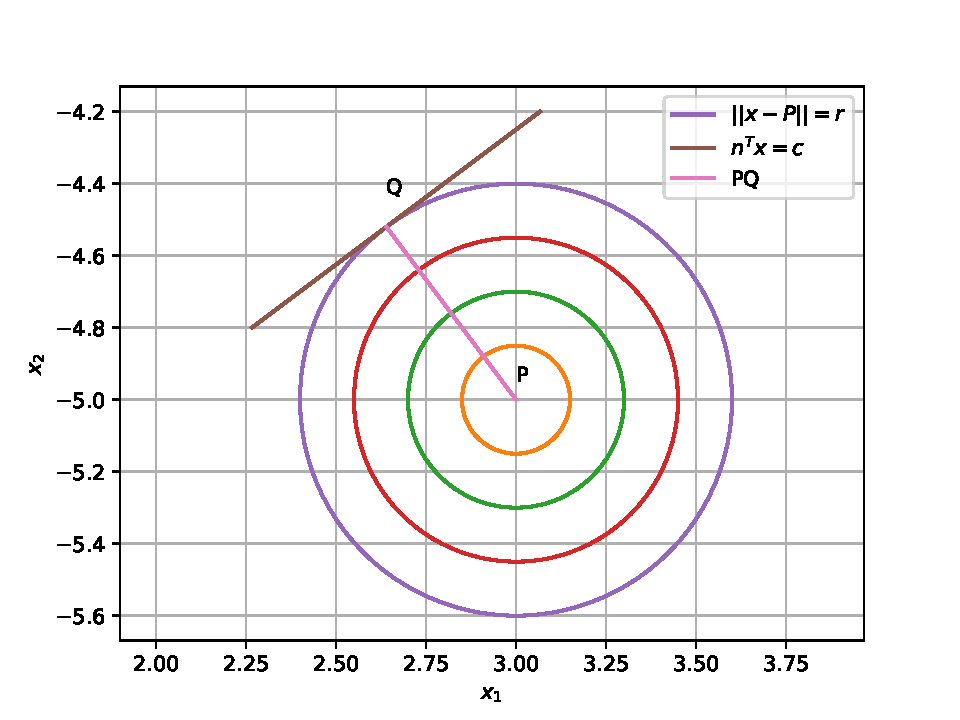
\includegraphics[width=\columnwidth]{./figs/opt/concirc.eps}
\caption{ Finding $ \displaystyle \min_{\mbf{x}}g\brak{\mbf{x}}$}.
\label{fig:concirc}	
\end{figure}
%
\item By solving the quadratic equation obtained from \eqref{eq:opt_line_nor_h},
show that 
\label{prob:minr}
\begin{align}
\min_{\vec{x}} r = \frac{3}{5}, \vec{x}_{\min} = \vec{Q}  = \myvec{2.64\\-4.52}
\end{align}
%
%and find $,
%$ that minimizes $r$. By labeling  $\vec{Q}$ 
In Fig. \ref{fig:concirc}, it can be seen  that $\vec{Q}$ is the point of contact of the line $L$ with the circle of minimum radius $r = \frac{3}{5}$.
%Obtain a theoretical solution for problem \ref{convex_code} 
%%using coordinate geometry.
%
%\solution 
%From \eqref{eq2_1_line} and \eqref{eq2_1_circ}, 
%%
%\begin{align}
%r^2 & = (x_1-8)^2 + (3- x_1)^2 \\
%&= 2 x_1^2 - 22 x_1 + 73 \\
%\Rightarrow r^2 &= \frac{\brak{2x_1-11}^2 + 5^2}{2}
%\end{align}
%%
%which is minium when $x_1 = \frac{11}{2}, x_2 = \frac{7}{2}$.  The minimum value is $\frac{25}{2}$ and 
%the radius $r = \frac{5}{\sqrt{2}}$.
\item Show that 
\begin{align}
\label{eq:lagrange_n}
\nabla h(\vec{x}) =  \myvec{3 \\ -4} = \vec{n}
\end{align}
where
\begin{equation}
\nabla =  
\begin{pmatrix}
\frac{\partial}{\partial x_1} \\
\frac{\partial}{\partial x_2} 
\end{pmatrix}
\end{equation}

\item Show that 
\begin{align}
\nabla g(\vec{x}) = 2\cbrak{\vec{x}-\myvec{3 \\ -5}} = 2\cbrak{\vec{x}-\vec{P}}
\label{eq:lagrange_pq}
\end{align}
%
%is the direction vector of the normal at $\vec{x}$.
\item From Fig. \ref{fig:concirc}, show that 
\begin{align}
\label{eq:opt_normal}
\nabla g(\vec{Q}) = \lambda \nabla h(\vec{Q}),
\end{align}
%
\solution In Fig. \ref{fig:concirc}, PQ is the normal to the line $L$, represented by $h\brak{\vec{x}}$. 
$\because$ the normal vector of $L$ is in the same direction as $PQ$,  for some constant $k$, 
%
\begin{align}
%\label{eq:opt_normal}
\brak{\vec{Q}-\vec{P}} = k \vec{n}
\end{align}
%
which is the same as \eqref{eq:opt_normal} after substituting from \eqref{eq:lagrange_n}.
 and \eqref{eq:lagrange_pq}.
%where $\vec{p}$ is the point of contact.
\item Use \eqref{eq:opt_normal} and $\vec{h(\vec{Q})}=0$ from \eqref{eq2_1_line} to obtain $\vec{Q}$.
\\
\solution From the given equations, we obtain
\begin{align}
\brak{\vec{Q}-\vec{P}}-\lambda \vec{n} &= 0 
\\
\vec{n}^T\vec{Q} - c &= 0
\label{eq:lagrange_mat_eq}
\end{align}
%
which can be simplifed to obtain
%
\begin{align}
\myvec{\vec{I} & -\vec{n} \\ \vec{n}^T & 0}\myvec{\vec{Q}\\ \lambda} = \myvec{\vec{P}\\c}
%\vec{Q} = \vec{P}+\frac{\brak{c-\vec{n}^T\vec{P}}}{\norm{\vec{n}}^2}\vec{n}
\label{eq:lagrange_mat_sol}
\end{align}
The following code computes the solution to \eqref{eq:lagrange_mat_sol}
%
\begin{lstlisting}
codes/opt/lagmul.py
\end{lstlisting}

\item
\label{lagrange}
	Define 
	\begin{equation}
	\label{lagrangian}
	C\brak{\mbf{x},\lambda} = g\brak{\mbf{x}} - \lambda h\brak{\mbf{x}}%, \quad \lambda > 0
	\end{equation}
and show that $\vec{Q}$ can also be obtained by 
solving the equations
%
\begin{align}
\nabla C\brak{\mbf{x},\lambda} &= 0.
\label{tangent}
\end{align}
%
What is the sign of $\lambda$?  $C$ is known as the Lagrangian and the above technique is known as the Method of Lagrange Multipliers.

%\solution
%From \eqref{eq2_1_line} and \eqref{eq2_1_circ}, 
%%
%\begin{align}
%L\brak{\mbf{x},\lambda} &= (x_1-8)^2 + (x_2-6)^2 - \lambda \brak{x_1 + x_2 - 9} \\
%\Rightarrow \nabla L\brak{\mbf{x},\lambda}  & = 
%\begin{pmatrix}
%2x_1  - 16 - \lambda \\
%2x_2 - 12 - \lambda \\
%x_1 + x_2 -9
%\end{pmatrix}
%\\
%&=
%\begin{pmatrix}
%2 &0 & - 1 \\
%0 &2 & - 1 \\
%1 & 1 & 0 
%\end{pmatrix}
%\begin{pmatrix}
%x_1 \\
%x_2 \\
%\lambda
%\end{pmatrix}
%= 
%\begin{pmatrix}
%16 \\
% 12 \\
%9
%\end{pmatrix}
%=
%0 
%\\
%\Rightarrow 
%\begin{pmatrix}
%x_1 \\
%x_2 \\
%\lambda
%\end{pmatrix}
%&= 
%\begin{pmatrix}
%\frac{11}{2} \\
% \frac{7}{2} \\
%-5
%\end{pmatrix}
%\end{align}
%%
%using the following python script.  Note that this method yields the same result as the previous exercises.  Thus, $\lambda$ is negative.
%	
\item Obtain $\vec{Q}$ using gradient descent.
\\
\solution
\begin{lstlisting}
codes/opt/gd_lagrange.py
\end{lstlisting}



\end{enumerate}

\section{KKT Conditions}
\subsection{Equality Constraints}

\begin{enumerate}[label=\thesubsection.\arabic*,ref=\thesubsection.\theenumi]

\item
	\label{kkt-convex_code}
Find
\begin{align}
\label{kkt-eq2_1_circ}
	\min_{\mbf{x}}f\brak{\mbf{x}} = \norm{\vec{x}-\myvec{8\\6}}^2 = r^2 \\
\text{s.t.} \quad 	g\brak{\mbf{x}} = \myvec{1 & 1}\vec{x} - 9 = 0\label{kkt-eq2_1_line}
%	\quad g\brak{\mbf{x}} = x_1 + x_2 - 9 = 0
\end{align}
by plotting the circles $f\brak{\vec{x}}$
%
%\begin{equation}
% \norm{\vec{x}-\myvec{8\\6}}^2 =r^2
%%(x_1-8)^2 + (x_2-6)^2 = r^2
%\end{equation}
%
% $\mbf{x}= \myvec{x_1\\x_2}$, 
for different values of $r$ along with the line $g\brak{\mbf{x}}$.
%
%\begin{equation}
%\label{kkt-eq2_1_line}
%g\brak{\mbf{x}} = \myvec{1 & 1}\vec{x} - 9 = 0
%\end{equation} 
%
\\
\solution 
The following code plots Fig. \ref{kkt-fig.2.1}	

%	
\begin{lstlisting}
codes/kkt/2.1.py
\end{lstlisting}

%
\begin{figure}[!ht]
\centering
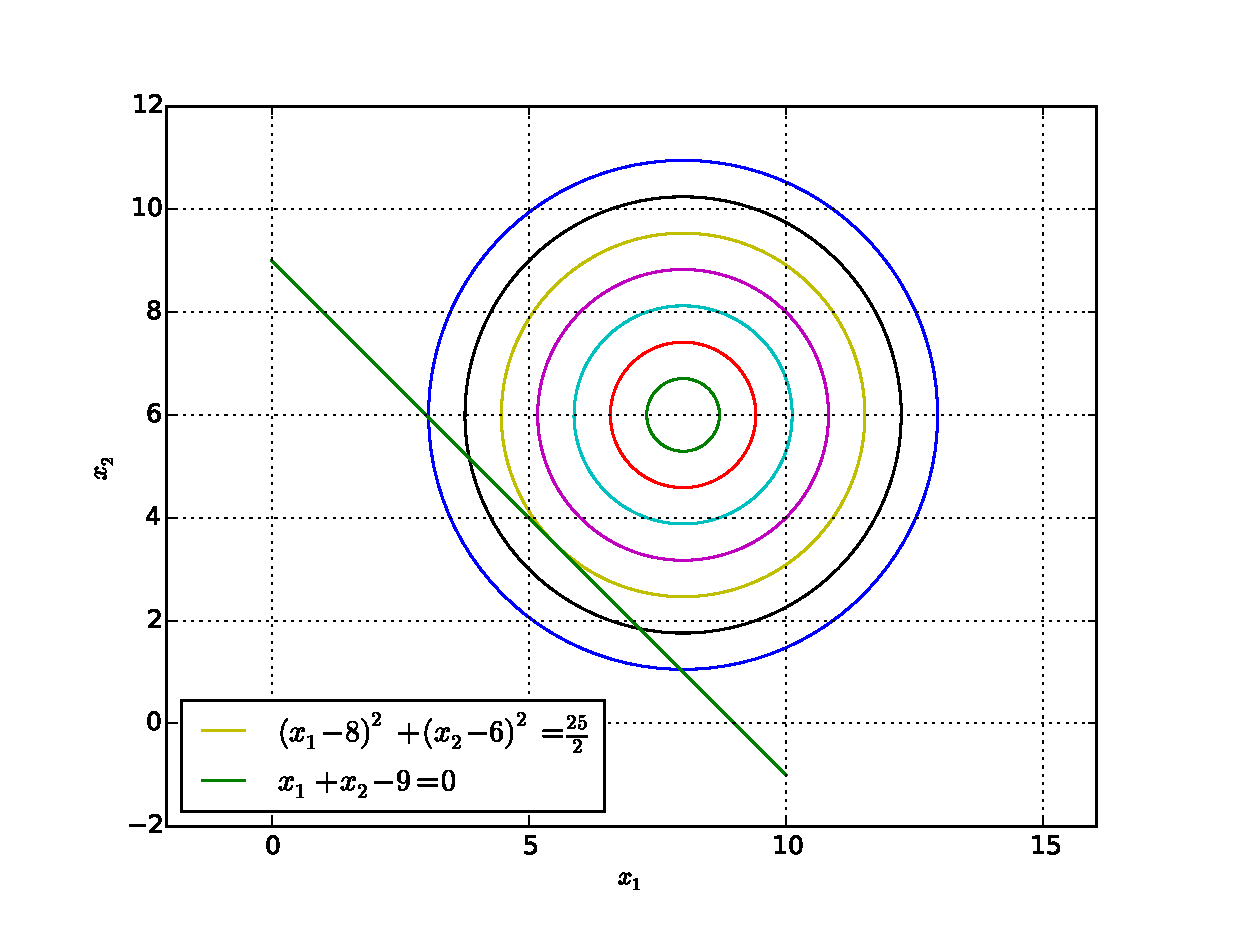
\includegraphics[width=\columnwidth]{./figs/kkt/2.1.eps}
\caption{ Finding $ \displaystyle \min_{\mbf{x}}f\brak{\mbf{x}}$}.
\label{kkt-fig.2.1}	
\end{figure}
%
\item Show that 
\begin{align}
\min r = \frac{5}{\sqrt{2}}
\end{align}
%Obtain a theoretical solution for problem \ref{kkt-convex_code} 
%%using coordinate geometry.
%
%\solution 
%From \eqref{kkt-eq2_1_line} and \eqref{kkt-eq2_1_circ}, 
%%
%\begin{align}
%r^2 & = (x_1-8)^2 + (3- x_1)^2 \\
%&= 2 x_1^2 - 22 x_1 + 73 \\
%\Rightarrow r^2 &= \frac{\brak{2x_1-11}^2 + 5^2}{2}
%\end{align}
%%
%which is minium when $x_1 = \frac{11}{2}, x_2 = \frac{7}{2}$.  The minimum value is $\frac{25}{2}$ and 
%the radius $r = \frac{5}{\sqrt{2}}$.
\item Show that 
\begin{align}
\nabla g(\vec{x}) = \myvec{1 \\ 1}
\end{align}
where
\begin{equation}
\nabla =  
\begin{pmatrix}
\frac{\partial}{\partial x_1} \\
\frac{\partial}{\partial x_2} 
\end{pmatrix}
\end{equation}

\item Show that 
\begin{align}
\nabla f(\vec{x}) = 2\cbrak{\vec{x}-\myvec{8 \\ 6}}
\end{align}
\item From Fig. \ref{kkt-fig.2.1}, show that 
\begin{align}
\label{kkt-eq:normal}
\nabla f(\vec{p}) = \lambda \nabla g(\vec{p}),
\end{align}
%
where $\vec{p}$ is the point of contact.
\item Use \eqref{kkt-eq:normal} and $\vec{g(p)}=0$ from \eqref{kkt-eq2_1_line} to obtain $\vec{p}$.
\item
\label{kkt-lagrange}
	Define 
	\begin{equation}
	\label{kkt-lagrangian}
	L\brak{\mbf{x},\lambda} = f\brak{\mbf{x}} - \lambda g\brak{\mbf{x}}%, \quad \lambda > 0
	\end{equation}
and show that $\vec{p}$ can also be obtained by 
solving the equations
%
\begin{align}
\nabla L\brak{\mbf{x},\lambda} &= 0.
\label{kkt-tangent}
\end{align}
%
What is the sign of $\lambda$?  $L$ is known as the Lagrangian and the above technique is known as the Method of Lagrange Multipliers.

\solution
%From \eqref{kkt-eq2_1_line} and \eqref{kkt-eq2_1_circ}, 
%%
%\begin{align}
%L\brak{\mbf{x},\lambda} &= (x_1-8)^2 + (x_2-6)^2 - \lambda \brak{x_1 + x_2 - 9} \\
%\Rightarrow \nabla L\brak{\mbf{x},\lambda}  & = 
%\begin{pmatrix}
%2x_1  - 16 - \lambda \\
%2x_2 - 12 - \lambda \\
%x_1 + x_2 -9
%\end{pmatrix}
%\\
%&=
%\begin{pmatrix}
%2 &0 & - 1 \\
%0 &2 & - 1 \\
%1 & 1 & 0 
%\end{pmatrix}
%\begin{pmatrix}
%x_1 \\
%x_2 \\
%\lambda
%\end{pmatrix}
%= 
%\begin{pmatrix}
%16 \\
% 12 \\
%9
%\end{pmatrix}
%=
%0 
%\\
%\Rightarrow 
%\begin{pmatrix}
%x_1 \\
%x_2 \\
%\lambda
%\end{pmatrix}
%&= 
%\begin{pmatrix}
%\frac{11}{2} \\
% \frac{7}{2} \\
%-5
%\end{pmatrix}
%\end{align}
%%
%using the following python script.  Note that this method yields the same result as the previous exercises.  Thus, $\lambda$ is negative.
%	
\begin{lstlisting}
codes/kkt/2.3.py
\end{lstlisting}
\end{enumerate}

\subsection{Inequality Constraints}


\begin{enumerate}[label=\thesubsection.\arabic*,ref=\thesubsection.\theenumi]
%
\item
\label{kkt-ch2_constraint}
Modify the code in problem \ref{kkt-convex_code} to find a graphical solution for minimising
\begin{align}
f\brak{\mbf{x}} 
%= (x_1-8)^2 + (x_2-6)^2
\end{align}
with constraint
\begin{align}
%\label{kkt-convex-constraint}
g\brak{\mbf{x}} \geq 0
%= x_1 + x_2 - 9 
\end{align}

\solution 
This problem reduces to finding the radius of the smallest circle in the shaded area in Fig. \ref{kkt-fig.2.4} .  It is clear that this radius is 0.
%	
\begin{lstlisting}
codes/kkt/2.4.py
\end{lstlisting}

%
\begin{figure}[!ht]
\centering
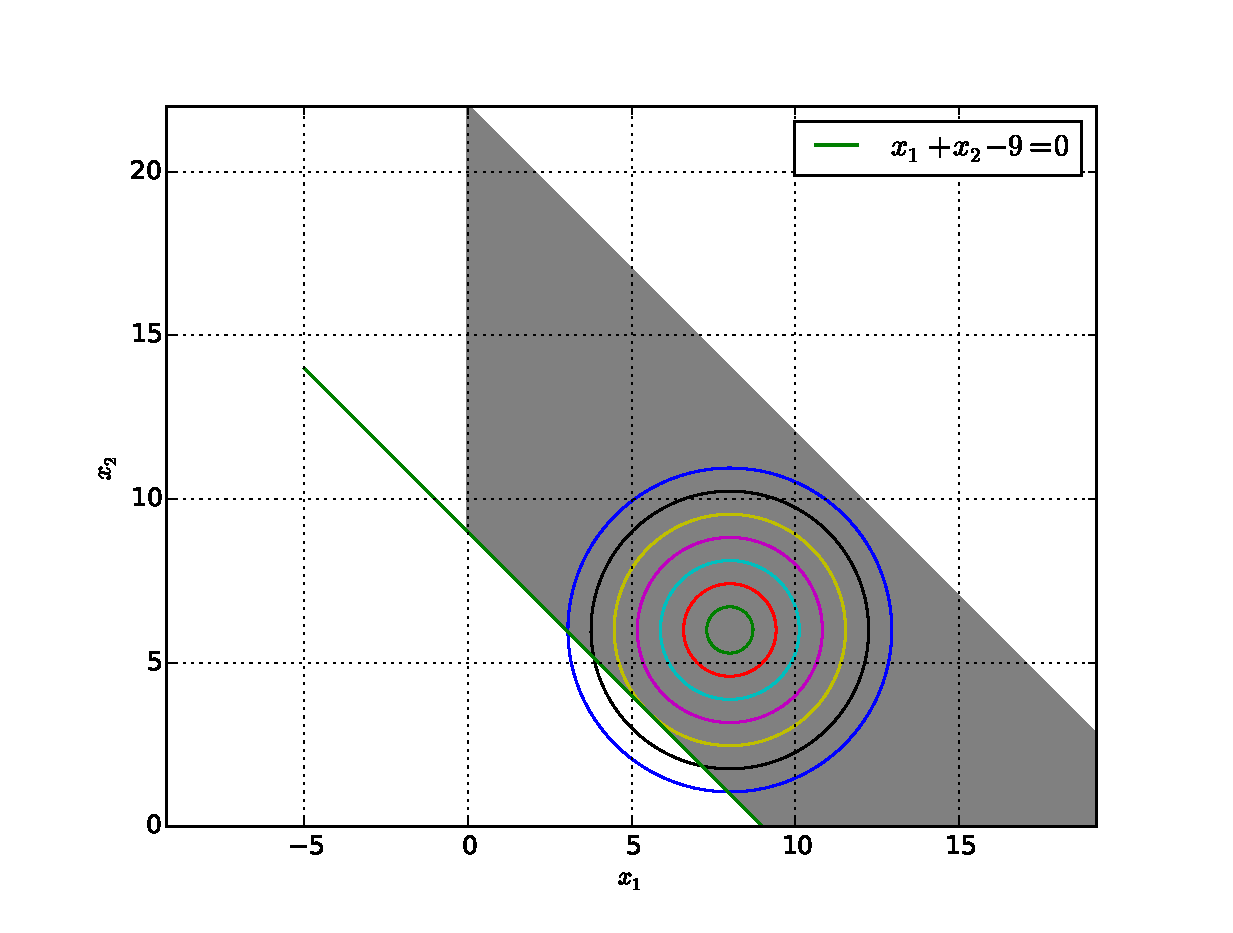
\includegraphics[width=\columnwidth]{./figs/kkt/2.4.eps}
\caption{ Smallest circle in the shaded region is a point.}
\label{kkt-fig.2.4}	
\end{figure}
%
\item
\label{kkt-ch2_lagrange_fail}
Now use the method of Lagrange multipliers to solve  problem \ref{kkt-ch2_constraint} and compare with the graphical solution.  Comment.

%
\solution Using the method of Lagrange multipliers, the solution is the same as the one obtained in  problem \ref{kkt-ch2_constraint}, which is different from the graphical solution.  This means that the Lagrange multipliers method cannot be applied blindly.
\item
Repeat problem \ref{kkt-ch2_lagrange_fail} by keeping 
 $\lambda=0$.   Comment.

\solution Keeping $\lambda = 0$ results in $\vec{x}=\myvec{ 8\\ 6}$, which is the correct solution.  The minimum value of $f\brak{\mbf{x}}$ without any constraints lies in the region $g\brak{\mbf{x}} = 0$.  In this case, $\lambda = 0$.  
%
%
\item
\label{kkt-ch2_constraint_border}
Find a graphical solution for minimising
\begin{align}
f\brak{\mbf{x}}
% = (x_1-8)^2 + (x_2-6)^2
\end{align}
with constraint
\begin{align}
%\label{kkt-convex-constraint}
g\brak{\mbf{x}} \leq 0
%= x_1 + x_2 - 9 .
\end{align}
Summarize your observations.

%
\solution In Fig. \ref{kkt-fig.2.7}, the shaded region represents the constraint.  Thus, the solution is the same as the one in problem \ref{kkt-ch2_constraint}. This implies that the method of
Lagrange multipliers can be used to solve the optimization problem with this inequality constraint as well.  Table \ref{kkt-table.2.7} summarizes the conditions for this based on the observations so far.
\begin{lstlisting}
codes/kkt/2.7.py
\end{lstlisting}
\begin{table}[!h]
\centering
%%%%%%%%%%%%%%%%%%%%%%%%%%%%%%%%%%%%%%%%%%%%%%%%%%%%%%%%%%%%%%%%%%%%%%
%%                                                                  %%
%%  This is the header of a LaTeX2e file exported from Gnumeric.    %%
%%                                                                  %%
%%  This file can be compiled as it stands or included in another   %%
%%  LaTeX document. The table is based on the longtable package so  %%
%%  the longtable options (headers, footers...) can be set in the   %%
%%  preamble section below (see PRAMBLE).                           %%
%%                                                                  %%
%%  To include the file in another, the following two lines must be %%
%%  in the including file:                                          %%
%%        \def\inputGnumericTable{}                                 %%
%%  at the beginning of the file and:                               %%
%%        \input{name-of-this-file.tex}                             %%
%%  where the table is to be placed. Note also that the including   %%
%%  file must use the following packages for the table to be        %%
%%  rendered correctly:                                             %%
%%    \usepackage[latin1]{inputenc}                                 %%
%%    \usepackage{color}                                            %%
%%    \usepackage{array}                                            %%
%%    \usepackage{longtable}                                        %%
%%    \usepackage{calc}                                             %%
%%    \usepackage{multirow}                                         %%
%%    \usepackage{hhline}                                           %%
%%    \usepackage{ifthen}                                           %%
%%  optionally (for landscape tables embedded in another document): %%
%%    \usepackage{lscape}                                           %%
%%                                                                  %%
%%%%%%%%%%%%%%%%%%%%%%%%%%%%%%%%%%%%%%%%%%%%%%%%%%%%%%%%%%%%%%%%%%%%%%



%%  This section checks if we are begin input into another file or  %%
%%  the file will be compiled alone. First use a macro taken from   %%
%%  the TeXbook ex 7.7 (suggestion of Han-Wen Nienhuys).            %%
\def\ifundefined#1{\expandafter\ifx\csname#1\endcsname\relax}


%%  Check for the \def token for inputed files. If it is not        %%
%%  defined, the file will be processed as a standalone and the     %%
%%  preamble will be used.                                          %%
\ifundefined{inputGnumericTable}

%%  We must be able to close or not the document at the end.        %%
	\def\gnumericTableEnd{\end{document}}


%%%%%%%%%%%%%%%%%%%%%%%%%%%%%%%%%%%%%%%%%%%%%%%%%%%%%%%%%%%%%%%%%%%%%%
%%                                                                  %%
%%  This is the PREAMBLE. Change these values to get the right      %%
%%  paper size and other niceties.                                  %%
%%                                                                  %%
%%%%%%%%%%%%%%%%%%%%%%%%%%%%%%%%%%%%%%%%%%%%%%%%%%%%%%%%%%%%%%%%%%%%%%

	\documentclass[12pt%
			  %,landscape%
                    ]{report}
       \usepackage[latin1]{inputenc}
       \usepackage{fullpage}
       \usepackage{color}
       \usepackage{array}
       \usepackage{longtable}
       \usepackage{calc}
       \usepackage{multirow}
       \usepackage{hhline}
       \usepackage{ifthen}

	\begin{document}


%%  End of the preamble for the standalone. The next section is for %%
%%  documents which are included into other LaTeX2e files.          %%
\else

%%  We are not a stand alone document. For a regular table, we will %%
%%  have no preamble and only define the closing to mean nothing.   %%
    \def\gnumericTableEnd{}

%%  If we want landscape mode in an embedded document, comment out  %%
%%  the line above and uncomment the two below. The table will      %%
%%  begin on a new page and run in landscape mode.                  %%
%       \def\gnumericTableEnd{\end{landscape}}
%       \begin{landscape}


%%  End of the else clause for this file being \input.              %%
\fi

%%%%%%%%%%%%%%%%%%%%%%%%%%%%%%%%%%%%%%%%%%%%%%%%%%%%%%%%%%%%%%%%%%%%%%
%%                                                                  %%
%%  The rest is the gnumeric table, except for the closing          %%
%%  statement. Changes below will alter the table's appearance.     %%
%%                                                                  %%
%%%%%%%%%%%%%%%%%%%%%%%%%%%%%%%%%%%%%%%%%%%%%%%%%%%%%%%%%%%%%%%%%%%%%%

\providecommand{\gnumericmathit}[1]{#1} 
%%  Uncomment the next line if you would like your numbers to be in %%
%%  italics if they are italizised in the gnumeric table.           %%
%\renewcommand{\gnumericmathit}[1]{\mathit{#1}}
\providecommand{\gnumericPB}[1]%
{\let\gnumericTemp=\\#1\let\\=\gnumericTemp\hspace{0pt}}
 \ifundefined{gnumericTableWidthDefined}
        \newlength{\gnumericTableWidth}
        \newlength{\gnumericTableWidthComplete}
        \newlength{\gnumericMultiRowLength}
        \global\def\gnumericTableWidthDefined{}
 \fi
%% The following setting protects this code from babel shorthands.  %%
 \ifthenelse{\isundefined{\languageshorthands}}{}{\languageshorthands{english}}
%%  The default table format retains the relative column widths of  %%
%%  gnumeric. They can easily be changed to c, r or l. In that case %%
%%  you may want to comment out the next line and uncomment the one %%
%%  thereafter                                                      %%
\providecommand\gnumbox{\makebox[0pt]}
%%\providecommand\gnumbox[1][]{\makebox}

%% to adjust positions in multirow situations                       %%
\setlength{\bigstrutjot}{\jot}
\setlength{\extrarowheight}{\doublerulesep}

%%  The \setlongtables command keeps column widths the same across  %%
%%  pages. Simply comment out next line for varying column widths.  %%
\setlongtables

\setlength\gnumericTableWidth{%
	53pt+%
	58pt+%
	55pt+%
0pt}
\def\gumericNumCols{3}
\setlength\gnumericTableWidthComplete{\gnumericTableWidth+%
         \tabcolsep*\gumericNumCols*2+\arrayrulewidth*\gumericNumCols}
\ifthenelse{\lengthtest{\gnumericTableWidthComplete > \linewidth}}%
         {\def\gnumericScale{\ratio{\linewidth-%
                        \tabcolsep*\gumericNumCols*2-%
                        \arrayrulewidth*\gumericNumCols}%
{\gnumericTableWidth}}}%
{\def\gnumericScale{1}}

%%%%%%%%%%%%%%%%%%%%%%%%%%%%%%%%%%%%%%%%%%%%%%%%%%%%%%%%%%%%%%%%%%%%%%
%%                                                                  %%
%% The following are the widths of the various columns. We are      %%
%% defining them here because then they are easier to change.       %%
%% Depending on the cell formats we may use them more than once.    %%
%%                                                                  %%
%%%%%%%%%%%%%%%%%%%%%%%%%%%%%%%%%%%%%%%%%%%%%%%%%%%%%%%%%%%%%%%%%%%%%%

\ifthenelse{\isundefined{\gnumericColA}}{\newlength{\gnumericColA}}{}\settowidth{\gnumericColA}{\begin{tabular}{@{}p{53pt*\gnumericScale}@{}}x\end{tabular}}
\ifthenelse{\isundefined{\gnumericColB}}{\newlength{\gnumericColB}}{}\settowidth{\gnumericColB}{\begin{tabular}{@{}p{58pt*\gnumericScale}@{}}x\end{tabular}}
\ifthenelse{\isundefined{\gnumericColC}}{\newlength{\gnumericColC}}{}\settowidth{\gnumericColC}{\begin{tabular}{@{}p{55pt*\gnumericScale}@{}}x\end{tabular}}

\begin{tabular}[c]{%
	b{\gnumericColA}%
	b{\gnumericColB}%
	b{\gnumericColC}%
	}

%%%%%%%%%%%%%%%%%%%%%%%%%%%%%%%%%%%%%%%%%%%%%%%%%%%%%%%%%%%%%%%%%%%%%%
%%  The longtable options. (Caption, headers... see Goosens, p.124) %%            \\	%
 %\hline	% Across the top of the table.
%%  The rest of these options are table rows which are placed on    %%
%%  the first, last or every page. Use \multicolumn if you want.    %%

%%  Header for the first page.                                      %%
%	\multicolumn{3}{c}{The First Header} \\ \hline 
%	\multicolumn{1}{c}{colTag}	%Column 1
%	&\multicolumn{1}{c}{colTag}	%Column 2
%	&\multicolumn{1}{c}{colTag}	\\ \hline %Last column
%	\endfirsthead

%%  The running header definition.                                  %%
%	\hline
%	\multicolumn{3}{l}{\ldots\small\slshape continued} \\ \hline
%	\multicolumn{1}{c}{colTag}	%Column 1
%	&\multicolumn{1}{c}{colTag}	%Column 2
%	&\multicolumn{1}{c}{colTag}	\\ \hline %Last column
%	\endhead

%%  The running footer definition.                                  %%
%	\hline
%	\multicolumn{3}{r}{\small\slshape continued\ldots} \\
%	\endfoot

%%  The ending footer definition.                                   %%
%	\multicolumn{3}{c}{That's all folks} \\ \hline 
%	\endlastfoot
%%%%%%%%%%%%%%%%%%%%%%%%%%%%%%%%%%%%%%%%%%%%%%%%%%%%%%%%%%%%%%%%%%%%%%

\hhline{|-|-|-}
	 \multicolumn{1}{|p{\gnumericColA}|}%
	{\gnumericPB{\centering}\textbf{Cost}}
	&\multicolumn{1}{p{\gnumericColB}|}%
	{\gnumericPB{\centering}\textbf{Constraint}}
	&\multicolumn{1}{p{\gnumericColC}|}%
	{\gnumericPB{\centering}\textbf{$\lambda$}}
\\
\hhline{|---|}
	 \multicolumn{1}{|p{\gnumericColA}|}%
	{\setlength{\gnumericMultiRowLength}{0pt}%
	 \addtolength{\gnumericMultiRowLength}{\gnumericColA}%
	 \multirow{3}[1]{\gnumericMultiRowLength}{\parbox{\gnumericMultiRowLength}{%
	 \gnumericPB{\centering}$f\brak{\mbf{x}}$}}}
	&\multicolumn{1}{p{\gnumericColB}|}%
	{\gnumericPB{\centering}$g\brak{\mbf{x}} = 0$}
	&\multicolumn{1}{p{\gnumericColC}|}%
	{\gnumericPB{\centering} $<$ 0}
\\
\hhline{~|--|}
	 \multicolumn{1}{|p{\gnumericColA}|}%
	{}
	&\multicolumn{1}{p{\gnumericColB}|}%
	{\gnumericPB{\centering}$g\brak{\mbf{x}} \geq 0 $}
	&\multicolumn{1}{p{\gnumericColC}|}%
	{\gnumericPB{\centering}0}
\\
\hhline{~|--|}
	 \multicolumn{1}{|p{\gnumericColA}|}%
	{}
	&\multicolumn{1}{p{\gnumericColB}|}%
	{\gnumericPB{\centering}$g\brak{\mbf{x}}\leq 0 $}
	&\multicolumn{1}{p{\gnumericColC}|}%
	{\gnumericPB{\centering} $<$ 0}
\\
\hhline{|-|-|-|}
\end{tabular}

\ifthenelse{\isundefined{\languageshorthands}}{}{\languageshorthands{\languagename}}
\gnumericTableEnd

	\caption{Summary of conditions.} 
\label{kkt-table.2.7}
\end{table}
%
\begin{figure}[!ht]
\centering
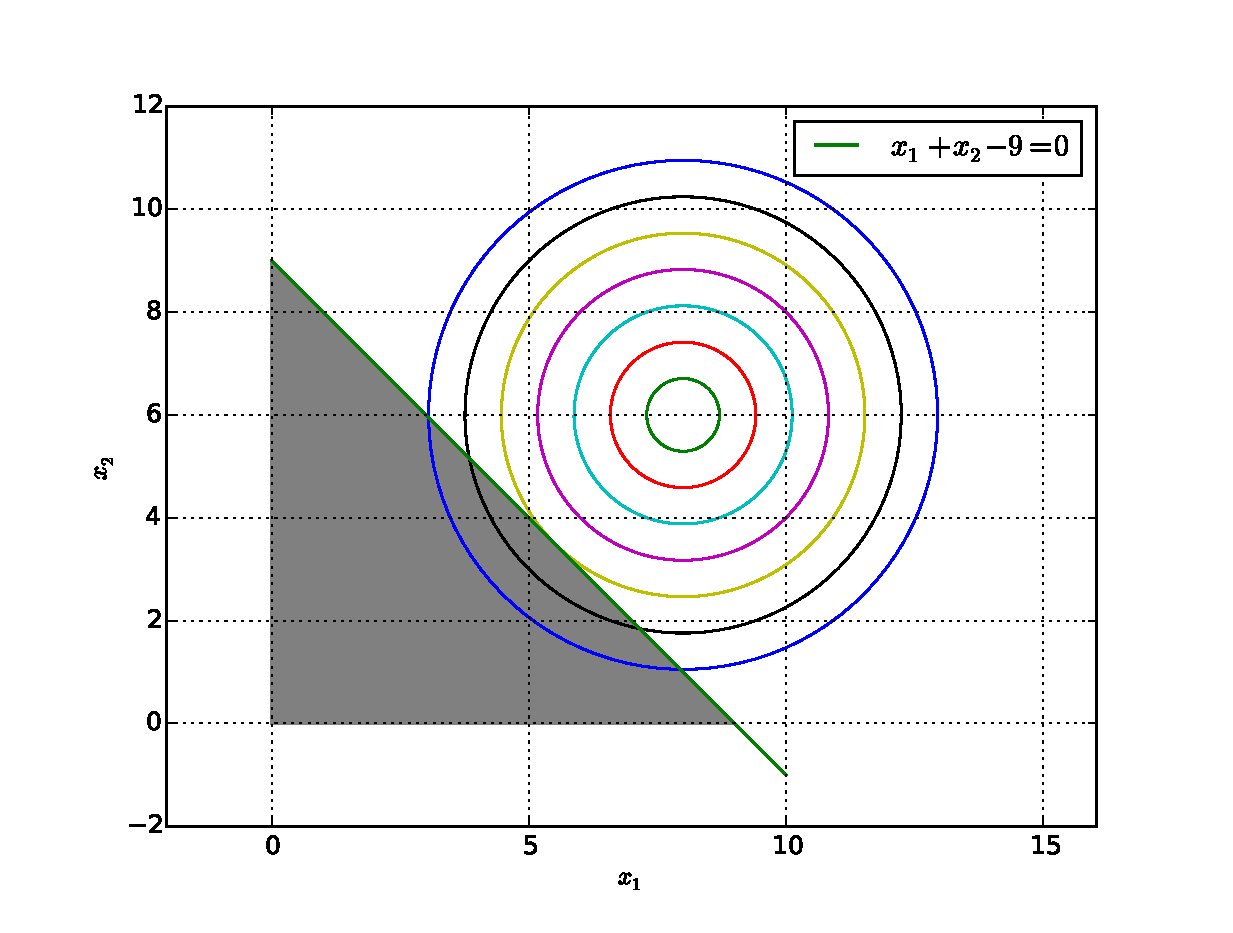
\includegraphics[width=\columnwidth]{./figs/kkt/2.7.eps}
\caption{ Finding $ \displaystyle \min_{\mbf{x}}f\brak{\mbf{x}}$.}
\label{kkt-fig.2.7}	
\end{figure}
%
\item
\label{kkt-ch2_prob_upper}
Find a graphical solution for 	 
	 \begin{align}
	 \label{kkt-ch2_second_min}
	\min_{\mbf{x}} f\brak{\mbf{x}} = \norm{\vec{x}-\myvec{8\\6}}^2
	 \end{align}
	 with constraint
	 \begin{align}
	 \label{kkt-ch2_second_const}
	 g\brak{\mbf{x}} = \myvec{1 & 1}\vec{x} - 18 = 0
	 \end{align}
	 
%
\solution
%	
\begin{lstlisting}
codes/kkt/2.8.py
\end{lstlisting}

%
\begin{figure}[!ht]
\centering
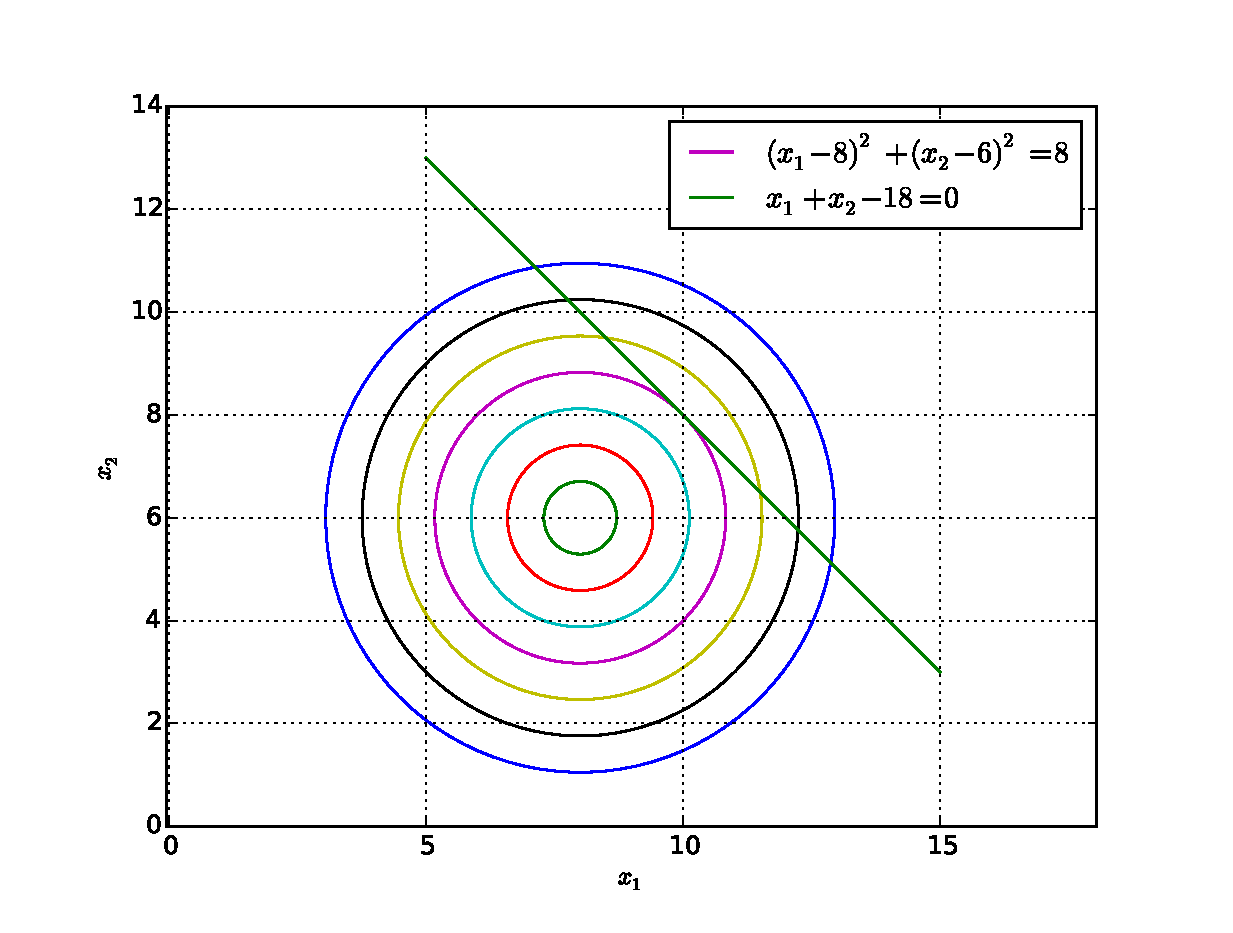
\includegraphics[width=\columnwidth]{./figs/kkt/2.8.eps}
\caption{ Finding $ \displaystyle \min_{\mbf{x}}f\brak{\mbf{x}}$.}
\label{kkt-fig.2.8}	
\end{figure}
%
\item
Repeat problem \ref{kkt-ch2_prob_upper} using the method of Lagrange mutipliers.  What is the sign of $\lambda$?

%
\solution
%From \eqref{kkt-ch2_second_min} and \eqref{kkt-ch2_second_const}, 
%%
%\begin{align}
%L\brak{\mbf{x},\lambda} &= (x_1-8)^2 + (x_2-6)^2 - \lambda \brak{x_1 + x_2 - 18} \\
%\Rightarrow \nabla L\brak{\mbf{x},\lambda}  & = 
%\begin{pmatrix}
%2x_1  - 16 - \lambda \\
%2x_2 - 12 - \lambda \\
%x_1 + x_2 -18
%\end{pmatrix}
%\\
%&=
%\begin{pmatrix}
%2 &0 & - 1 \\
%0 &2 & - 1 \\
%1 & 1 & 0 
%\end{pmatrix}
%\begin{pmatrix}
%x_1 \\
%x_2 \\
%\lambda
%\end{pmatrix}
%= 
%\begin{pmatrix}
%16 \\
% 12 \\
%18
%\end{pmatrix}
%=
%0 
%\\
%\Rightarrow 
%\begin{pmatrix}
%x_1 \\
%x_2 \\
%\lambda
%\end{pmatrix}
%&= 
%\begin{pmatrix}
%10 \\
% 8 \\
%4
%\end{pmatrix}
%\end{align}
%%
Using the following python script, $\lambda$ is positive and the minimum value of $f$ is 8.
%	
\begin{lstlisting}
codes/kkt/2.9.py
\end{lstlisting}

%
%
\item
\label{kkt-ch2_prob_upper_cond}
Solve
	 \begin{align}
%	 \label{kkt-ch2_second_min}
	\min_{\mbf{x}} f\brak{\mbf{x}} 
%= (x_1-8)^2 + (x_2-6)^2
	 \end{align}
	 with constraint
	 \begin{align}
%	 \label{kkt-ch2_second_const}
	 g\brak{\mbf{x}} 
%= x_1 + x_2 - 18 
\geq 0 
	 \end{align}
	 
%
\solution Since the unconstrained solution is outside the region $g\brak{\mbf{x}} \geq 0$, the solution is the same as the one in problem \ref{kkt-ch2_prob_upper}.
%
\item
Based on the problems so far, generalise the Lagrange multipliers method for 
%
	 \begin{align}
	 \label{kkt-ch2_lagrange_ineq}
	\min_{\mbf{x}} f\brak{\mbf{x}} , \quad 
	 g\brak{\mbf{x}}  \geq 0 
	 \end{align}
%

%
\solution
Considering $L\brak{\mbf{x},\lambda} = f\brak{\mbf{x}} - \lambda g\brak{\mbf{x}}$, for $g\brak{\mbf{x}} = \myvec{1 & 1}\vec{x} - 18 \geq 0$ we found $\lambda > 0 $ and for $g\brak{\mbf{x}} = \myvec{1 & 1}\vec{x} - 9 \leq 0, \lambda < 0$. A single condition can be obtained by framing the optimization problem as
%
	 \begin{align}
	 \label{kkt-ch2_lagrange_ineq_summary}
	\min_{\mbf{x}} f\brak{\mbf{x}} , \quad 
	 g\brak{\mbf{x}}  \leq 0 
	 \end{align}
%
with the Lagrangian
%
\begin{equation}
%\label{kkt-ch2_kkt_necessary}
L\brak{\mbf{x},\lambda} = f\brak{\mbf{x}} + \lambda g\brak{\mbf{x}}, %\quad  \lambda > 0,  g\brak{\mbf{x}} \leq 0.
\end{equation}
%
provided
%
\begin{equation}
\label{kkt-ch2_kkt_necessary}
\nabla L\brak{\mbf{x},\lambda} = 0 \Rightarrow \lambda > 0
\end{equation}
else, $\lambda = 0$.
\end{enumerate}

\subsection{Karush Kuhn-Tucker Conditions}

\begin{enumerate}[label=\thesubsection.\arabic*,ref=\thesubsection.\theenumi]
\item
Solve
 \begin{align}
 \label{kkt-ch2_kkt_problem}
\min_{\mbf{x}} f\brak{\mbf{x}} = \vec{x}^T\myvec{4 & 0 \\0 & 2}\vec{x}
%4x_1^2 + 2x_2^2
 \end{align}
 with constraints
 \begin{align}
 g_1\brak{\mbf{x}} = \myvec{3 & 1}\vec{x}-8 = 0\\
 g_2 \brak{\mbf{x}}= 15 - \myvec{2 & 4}\vec{x} \geq 0
 \end{align}
 
%
\solution Considering the Lagrangian
%
\begin{align}
%L\brak{\mbf{x},\lambda} &= f\brak{\mbf{x}} + \lambda g_1\brak{\mbf{x}} - \mu g_2\brak{\mbf{x}} \\
% &= 4x_1^2 + 2x_2^2 + \lambda \brak{3x_1 + x_2-8} 
% \nonumber \\
% &\,-\mu\brak{15 - 2x_1 - 4x_2},\\
 \nabla L\brak{\mbf{x},\lambda, \mu}  %& = 
%\begin{pmatrix}
%8x_1 + 3 \lambda  +2 \mu  \\
%4x_2 + \lambda + 4 \mu \\
%3x_1 + x_2 -8 \\
% - 2x_1 - 4x_2 + 15
%\end{pmatrix}
= 0
\end{align}
%
resulting in the matrix equation
%
\begin{align}
\Rightarrow 
\begin{pmatrix}
8 &0 & 3 & 2\\
0 &4 & 1 & 4 \\
3 & 1 & 0 &0  \\
2 & 4 & 0 & 0
\end{pmatrix}
\begin{pmatrix}
x_1 \\
x_2 \\
\lambda
\\
\mu
\end{pmatrix}
&=
\begin{pmatrix}
0 \\
0 \\
8 \\
15
\end{pmatrix}
\\
\Rightarrow 
\begin{pmatrix}
x_1 \\
x_2 \\
\lambda
\\
\mu
\end{pmatrix}
&= 
\begin{pmatrix}
1.7 \\
 2.9 \\
-3.12 \\
-2.12
\end{pmatrix}
\end{align}
%
using the following python script.  The (incorrect) graphical solution is available in Fig. \ref{kkt-fig.2.12}
%	
\begin{lstlisting}
codes/kkt/2.12.py
\end{lstlisting}

%
Note that $\mu < 0 $, contradicting the necessary condition in \eqref{kkt-ch2_kkt_necessary}. 
%
\begin{figure}[!ht]
\centering
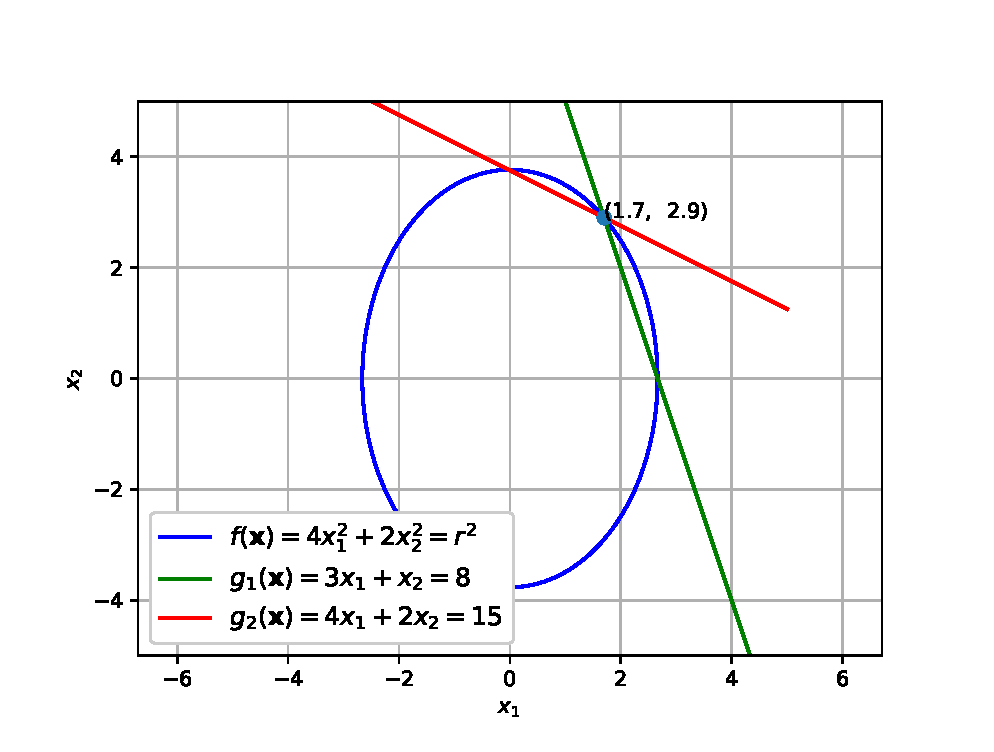
\includegraphics[width=\columnwidth]{./figs/kkt/2.12_1.eps}
\caption{ Incorrect solution is at intersection of all curves $r = 5.33$}
\label{kkt-fig.2.12}	
\end{figure}
\item
Obtain the correct solution to the previous problem by considering $\mu = 0$.

\begin{figure}[!ht]
\centering
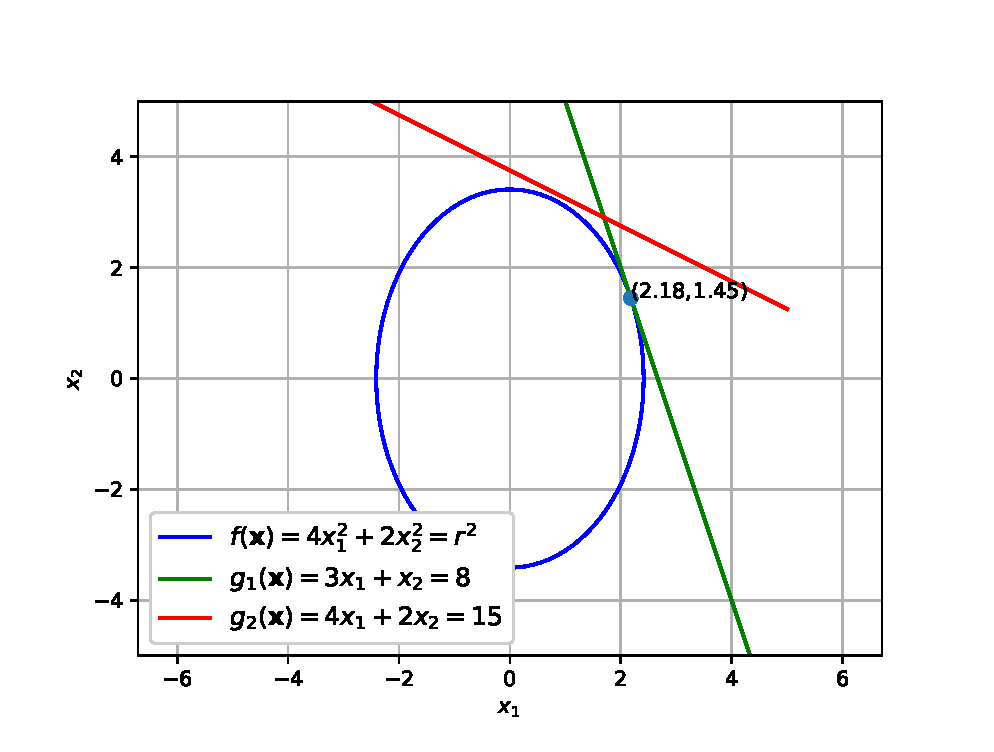
\includegraphics[width=\columnwidth]{./figs/kkt/2.12_2.eps}
\caption{ Optimal solution is where $g_1(x)$ touches the curve $r = 4.82$}
\label{kkt-fig.2.13}	
\end{figure}
%
%
\item
Solve
 \begin{align}
% \label{kkt-ch2_kkt_problem}
\min_{\mbf{x}} f\brak{\mbf{x}} %= 4x_1^2 + 2x_2^2
 \end{align}
 with constraints
 \begin{align}
 g_1\brak{\mbf{x}} 
%= 3x_1 + x_2-8 
= 0\\
 g_2 \brak{\mbf{x}}
%= 15 - 2x_1 - 4x_2 
\leq 0
 \end{align}
 
%
\item
Based on whatever you have done so far,	list the steps that you would use in general for solving a convex optimization problem  like \eqref{kkt-ch2_kkt_problem}  using Lagrange Multipliers. 
These are called Karush-Kuhn-Tucker(KKT) conditions.

\solution For a problem defined by 
\begin{align}
\mbf{x^*} &= \min_{\mbf{x}}f(\mbf{x})
\\
\text{subject to } h_i(\mbf{x}) &= 0, \forall i=1,..,m
\\
\text{subject to } g_i(\mbf{x}) &\le 0, \forall i=1,..,n
\end{align}
%
the optimal solution is obtained through
%
\begin{align}
\mbf{x^*} &= \min_{\mbf{x}}L(\mbf{x}, \mbf{\lambda}, \mbf{\mu}) 
\\
&= \min_{\mbf{x}}f(\mbf{x})  + \underset{i=1}{\overset{m}{\sum}} \lambda_i h_i(\mbf{x}) + \underset{i=1}{\overset{n}{\sum}} \mu_i g_i(\mbf{x}),
\end{align}
%
using the KKT conditions
%
\begin{align}
\Rightarrow \nabla_\mbf{x} f(\mbf{x})  + \underset{i=1}{\overset{m}{\sum}} \nabla_\mbf{x} \lambda_i h_i(\mbf{x}) + \underset{i=1}{\overset{n}{\sum}} \mu_i \nabla_\mbf{x} g_i(\mbf{x}) = 0 
\\
\text{subject to }\mu_i g_i(\mbf{x}) = 0, \forall i = 1,..,n
\\
\text{and }\mu_i \ge 0, \forall i = 1,..,n
\end{align}
%
\item
	Maxmimize 
	%
	\begin{align}
	f(\mbf{x}) &= \sqrt{x_1x_2}
	\end{align}
	%
	with the constraints
	%
	\begin{align}
	x_1^2+x_2^2 &\leq 5 \\
	x_1 \geq 0, x_2 &\geq 0
	\end{align}
	%

%
\item
	\label{kkt-convex_sdp_eqiv}
	%
	Solve
	\begin{equation}
	\min_{\mbf{x}} \quad x_1 + x_2
	\end{equation}
	%	
	with the constraints
	\begin{equation}
	x_1^2 - x_1 + x_2^2 \leq 0
	\end{equation}
	%
where 
$
\mbf{x} = \begin{pmatrix}
x_1 \\
x_2
\end{pmatrix}
$

\solution 
%Using the method of Lagrange multipliers,
%%
%\begin{align}
%\label{kkt-ch2_sd_kkt}
%\nabla \cbrak{f(\mbf{x})  +  \mu g(\mbf{x}) }= 0 , \quad \mu \ge 0
%\end{align}
%%
%resulting in the equations
%%
%\begin{align}
%2x_1\mu -\mu + 1 &= 0 \\
%2x_2\mu + 1 &=0 \\
%x_1^2 -x_1 + x_2^2 &= 0 
%\end{align}
%%
%which can be simplified to obtain 
%%
%\begin{align}
%\brak{\frac{1-\mu}{2\mu}}^2 + \brak{\frac{1}{2\mu}}^2 + \frac{1-\mu}{2\mu} &= 0 \\
%\Rightarrow 1 + \mu^2 -2\mu + 1 + 2\mu\brak{1-\mu} &= 0 \\
%\Rightarrow \mu^2 =2, or \mu &= \pm \sqrt{2} 
%\end{align}
%%
%From \eqref{kkt-ch2_kkt_problem},  $\mu \ge 0 \Rightarrow  \mu = \sqrt{2}$. The desired solution is
%%
%\begin{equation}
%\mbf{x} = 
%\begin{pmatrix}
% \frac{\sqrt{2}-1}{2\sqrt{2}} \\
%-\frac{1}{2\sqrt{2}} 
%\end{pmatrix}
%\end{equation}
%
\\
{\em Graphical solution:} 
%The constraint can be expressed as
%%
%\begin{align}
%x_1^2 - x_1 + x_2^2 &\le 0 \\
%\Rightarrow \brak{x_1 - \frac{1}{2}}^2 + x_2^2 & \le \brak{\frac{1}{2}}^2
%\end{align}
%
%	
\begin{lstlisting}
codes/kkt/2.15.py
\end{lstlisting}

%
%
\begin{figure}[!ht]
\centering
\includegraphics[width=\columnwidth]{./figs/kkt/2.15.eps}
\caption{ Optimal solution is the lower tangent to the circle}
\label{kkt-fig.2.15}	
\end{figure}
%
\end{enumerate}


\section{
	Quadratic Programming
}

%\renewcommand{\theequation}{\theenumi}
\begin{enumerate}[label=\thesection.\arabic*.,ref=\thesection.\theenumi]
\numberwithin{equation}{enumi}

\item An apache helicopter of the enemy is flying along the curve given by 
	\label{prob:dist_pt_parab}
\begin{align}
\label{eq:dist_pt_parab}
y = x^2 +7
\end{align}
%
A soldier, placed at 
\begin{align}
\vec{P} = \myvec{3\\7}.  
\end{align}
%
wants to shoot the heicopter when it is nearest to him.  Express this as an optimization problem.
%\item
%Express the problem of 
%finding the point on the curve 
%\begin{align}
%\label{eq:dist_pt_parab}
%x^2 = 2y
%\end{align}
%%
%nearest to the point 
%\begin{align}
%\vec{P} = \myvec{0\\5}.  
%\end{align}
%%
%as an optiimization problem.
\\
\solution The given problem can be expressed as
\begin{align}
\label{eq:qp_dist_pt_parab}
\min_{\vec{x}}\norm{\vec{x}-\vec{P}}^2
\\
\text{s.t. }\vec{x}^T\vec{V}\vec{x} + \vec{u}^T\vec{x}  +d = 0
\end{align}
%
where
%
\begin{align}
\vec{V} &= \myvec{1 & 0\\0 & 0}
\\
\vec{u} &= -\myvec{0 \\ 1}
\\
d &= 7
\end{align}
\item Show that the constraint in \ref{eq:qp_dist_pt_parab} is nonconvex.
\item Show that the following {\em relaxation} makes \eqref{eq:qp_dist_pt_parab} a convex optimization problem.
%
\begin{align}
\label{eq:qp_dist_pt_parab_conv}
\min_{\vec{x}}\brak{\vec{x}-\vec{P}}^T\brak{\vec{x}-\vec{P}}
\\
\text{s.t. }\vec{x}^T\vec{V}\vec{x} + \vec{u}^T\vec{x}  \le 0
\end{align}
%
%
\item Solve \eqref{eq:qp_dist_pt_parab_conv} using cvxpy.
\\
\solution  The following code yields the minimum distance as 2.236 and the nearest point on the curve as
%
\begin{align}
\vec{Q} &= \myvec{1\\8}
\end{align}

\begin{lstlisting}
codes/opt/qp_cvx.py
\end{lstlisting}

\item Solve \eqref{eq:qp_dist_pt_parab_conv} using the method of Lagrange multipliers.
\item Graphically verify the solution to Problem \ref{prob:dist_pt_parab}. 
%by drawing a figure.
\\
\solution 
The following code plots Fig. \ref{fig:qp_parab}
%	
\begin{lstlisting}
codes/opt/qp_parab.py
\end{lstlisting}

%
\begin{figure}[!ht]
\centering
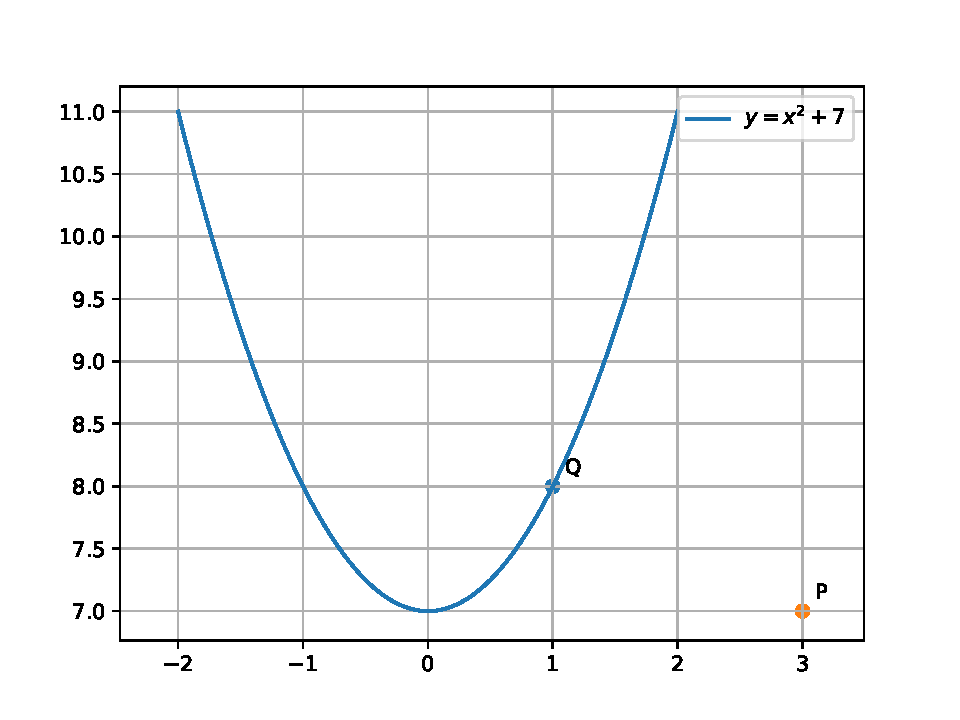
\includegraphics[width=\columnwidth]{./figs/opt/qp_parab.eps}
\caption{ $\vec{Q}$ is closest to $\vec{P}$}.
\label{fig:qp_parab}
\end{figure}
%
%\item Frame 	
% as an optimization problem.
%\label{prob:qp_dist_pt_parab}
%\\
%
%\solution 
%From \eqref{eq2_1_line} and \eqref{eq2_1_circ}, 
%%
%\begin{align}
%r^2 & = (x_1-8)^2 + (3- x_1)^2 \\
%&= 2 x_1^2 - 22 x_1 + 73 \\
%\Rightarrow r^2 &= \frac{\brak{2x_1-11}^2 + 5^2}{2}
%\end{align}
%%
%which is minium when $x_1 = \frac{11}{2}, x_2 = \frac{7}{2}$.  The minimum value is $\frac{25}{2}$ and 
%the radius $r = \frac{5}{\sqrt{2}}$.
%	
%\begin{lstlisting}
%codes/opt/optimization/lagmul.py
%\end{lstlisting}
\item Solve \eqref{eq:qp_dist_pt_parab_conv} using gradient descent.
%


\end{enumerate}


%\section{
%	Linear Programming
%}
%%\renewcommand{\theequation}{\theenumi}
%\begin{enumerate}[label=\thesection.\arabic*.,ref=\thesection.\theenumi]
%\numberwithin{equation}{enumi}

\section{Semi-definite Programming}

\begin{enumerate}[label=\thesection.\arabic*,ref=\thesection.\theenumi]


		\item
	\label{convex_sdp_eqiv}
	%
	Solve
	\begin{equation}
	\min_{\mbf{x}} \quad x_1 + x_2
	\end{equation}
	%	
	with the constraints
	\begin{equation}
	x_1^2 - x_1 + x_2^2 \leq 0
	\end{equation}
	%
where 
$
\mbf{x} = \begin{pmatrix}
x_1 \\
x_2
\end{pmatrix}
$

%\solution 
%Using the method of Lagrange multipliers,
%%
%\begin{align}
%\label{ch2_sd_kkt}
%\nabla \cbrak{f(\mbf{x})  +  \mu g(\mbf{x}) }= 0 , \quad \mu \ge 0
%\end{align}
%%
%resulting in the equations
%%
%\begin{align}
%2x_1\mu -\mu + 1 &= 0 \\
%2x_2\mu + 1 &=0 \\
%x_1^2 -x_1 + x_2^2 &= 0 
%\end{align}
%%
%which can be simplified to obtain 
%%
%\begin{align}
%\brak{\frac{1-\mu}{2\mu}}^2 + \brak{\frac{1}{2\mu}}^2 + \frac{1-\mu}{2\mu} &= 0 \\
%\Rightarrow 1 + \mu^2 -2\mu + 1 + 2\mu\brak{1-\mu} &= 0 \\
%\Rightarrow \mu^2 =2, or \mu &= \pm \sqrt{2} 
%\end{align}
%%
%From \eqref{ch2_kkt_problem},  $\mu \ge 0 \Rightarrow  \mu = \sqrt{2}$. The desired solution is
%%
%\begin{equation}
%\mbf{x} = 
%\begin{pmatrix}
% \frac{\sqrt{2}-1}{2\sqrt{2}} \\
%-\frac{1}{2\sqrt{2}} 
%\end{pmatrix}
%\end{equation}
%
%\\
%{\em Graphical solution:} 
%The constraint can be expressed as
%%
%\begin{align}
%x_1^2 - x_1 + x_2^2 &\le 0 \\
%\Rightarrow \brak{x_1 - \frac{1}{2}}^2 + x_2^2 & \le \brak{\frac{1}{2}}^2
%\end{align}
%
%	
%\begin{lstlisting}
%wget https://raw.githubusercontent.com/gadepall/optimization/master/manual/codes/2.15.py
%\end{lstlisting}

%
%
%\begin{figure}[!ht]
%\centering
%\includegraphics[width=\columnwidth]{./figs/2.15.eps}
%\caption{ Optimal solution is the lower tangent to the circle}
%\label{fig.2.15}	
%\end{figure}
%

%\subsection{Karush Kuhn-Tucker Conditions}

\item
%
\label{prob:cvxopt}

%\label{ch3_convex_ch2}
The problem
\begin{equation}
\min_{\mbf{X}} x_{11} + x_{12}
\end{equation}
%	
with constraints
\begin{align}
x_{11} + x_{22} &= 1 \\	
\mbf{X}
& \succeq 0 \quad  \brak{\text{$\succeq$ means positive definite}}
\end{align}
%
where
\begin{equation}
\mbf{X}=
\begin{pmatrix}
x_{11} & x_{12} \\
x_{12} & x_{22}
\end{pmatrix} 
\end{equation}
%
is known as a semi-definite program. 

%\solution The {\em cvxopt} solver needs to be used in order to find a numerical solution.  For this, the given problem has to be reformulated as
%\begin{align}
%&\min_{\mbf{x}}  
%\begin{pmatrix}
%1 & 1 & 0
%\end{pmatrix}
%\begin{pmatrix}
%x_{11} 
%\\
%x_{12}
%\\
%x_{22}
%\end{pmatrix}
%\quad \text{s.t}
%\\
%&
%\begin{pmatrix}
%1 & 0 & 1
%\end{pmatrix}
%\begin{pmatrix}
%x_{11} 
%\\
%x_{12}
%\\
%x_{22}
%\end{pmatrix}
%=1
%\end{align}
%\begin{multline}
%x_{11}
%\begin{pmatrix}
%-1 & 0 
%\\
%0 & 0
%\end{pmatrix}
%+
%x_{12}
%\begin{pmatrix}
%0 & -1
%\\
%-1 & 0
%\end{pmatrix}
%+x_{22}
%\begin{pmatrix}
%0 & 0 
%\\
%0 & -1
%\end{pmatrix}
%\\
%\preceq 
%\begin{pmatrix}
%0 & 0 
%\\
%0 & 0
%\end{pmatrix}.
%\end{multline}
%%
%The following script provides the solution to this problem.
%\begin{lstlisting}
%wget https://raw.githubusercontent.com/gadepall/optimization/master/manual/codes/3.1.py
%\end{lstlisting}
%
\item
Frame Problem \ref{prob:cvxopt} in terms of matrices.

\solution
It is easy to verify that
\begin{equation}
x_{11} + x_{12} = 
\begin{pmatrix}
1 & 1
\end{pmatrix}
\mbf{X}^{T}
\begin{pmatrix}
1 
\\
0
\end{pmatrix}
\end{equation}
and
\begin{equation}
x_{11} + x_{22} = 
\begin{pmatrix}
1 & 0 & 0 & 1
\end{pmatrix}
\begin{pmatrix}
\mbf{X} & \mbf{0} \\
\mbf{0} & \mbf{X}
\end{pmatrix}
\begin{pmatrix}
1
\\
0 
\\
0
\\
1
\end{pmatrix}
\end{equation}
%
Thus, Problem \ref{prob:cvxopt} can be expressed as
\begin{equation}
\begin{split}
\min_{\mbf{X}} 
\begin{pmatrix}
1 & 1
\end{pmatrix}
\mbf{X}^{T}
\begin{pmatrix}
1 
\\
0
\end{pmatrix}
& \quad s.t
\\
\begin{pmatrix}
1 & 0 & 0 & 1
\end{pmatrix}
\begin{pmatrix}
\mbf{X} & \mbf{0} \\
\mbf{0} & \mbf{X}
\end{pmatrix}
\begin{pmatrix}
1
\\
0 
\\
0
\\
1
\end{pmatrix}
&=1,
\\
\mbf{X}
 & \succeq 0 
\end{split}
\label{prob:cvxpy}
\end{equation}
%	
\item
Solve \eqref{prob:cvxpy} using {\em cvxpy}.
 Compare with the solution 
in problem  \ref{convex_sdp_eqiv}.

%
\solution
\begin{lstlisting}
wget https://raw.githubusercontent.com/gadepall/optimization/master/manual/codes/3.1-cvx.py
\end{lstlisting}

\item
Minimize 
\begin{equation}
-x_{11} - 2x_{12} - 5x_{22}
\end{equation}
subject to
\begin{align}
\label{ch3_lin_mat_ineq_const}
2x_{11} + 3x_{12} + x_{22} &= 7 \\
x_{11} + x_{12} &\geq 1 \\
x_{11}, x_{12}, x_{22} &\geq 0 \\
\begin{pmatrix}
x_{11} & x_{12} \\
x_{12} & x_{22}
\end{pmatrix} & \succeq 0 
\end{align}
using {\em cvxpy}.

%\solution
%In this problem, there is an SDP inequality and several linear inequalities.  The linear inequalities can be combined to obtain the matrix inequality
%%
%\begin{equation}
%\label{ch3_lin_mat_ineq}
%\begin{pmatrix}
%x_{11} + x_{12}- 1 & 0  & 0 & 0\\
%0 & x_{11} & 0 & 0
%\\
%0 & 0 & x_{12} &  0
%\\
 %0 & 0 & 0 & x_{22} 
%\end{pmatrix}
 %\succeq 0 
%\end{equation}
%%
%\eqref{ch3_lin_mat_ineq} can be combined with the matrix inequality in \eqref{ch3_lin_mat_ineq_const} to obtain the composite SDP
%\begin{equation}
%\label{ch3_lin_mat_sdp_ineq}
%\begin{pmatrix}
%\begin{matrix}
%x_{11} + x_{12}- 1 & 0  & 0 & 0\\
%0 & x_{11} & 0 & 0
%\\
%0 & 0 & x_{12} &  0
%\\
 %0 & 0 & 0 & x_{22} 
%\end{matrix}
%& \mbf{0}
%\\
%\mbf{0} & \begin{matrix}
%x_{11} & x_{12} \\
%x_{12} & x_{22}
%\end{matrix}
%\end{pmatrix} 
 %\succeq 0 
%\end{equation}
%%
%For using  {\em cvxpy}, the SDP in \eqref{ch3_lin_mat_sdp_ineq} can be expressed as
%%
%\begin{equation}
 %x_{11}F_{0} + x_{12}F_1+x_{22}F_{2}\succeq B ,
%\end{equation}
%%
%where
%%
%\begin{align}
%F_{0} = 
%\begin{pmatrix}
%\begin{matrix}
%1 &
%\\
%& 1
%\end{matrix}
%& & \bigzero
%\\
%& 
%\begin{matrix}
%0 &
%\\
%& 0
%\end{matrix}
%&
%\\
%\bigzero& & 
 %\begin{matrix}
%1 &  \\
 %& 0
%\end{matrix}
%\end{pmatrix} 
%\\
%F_{1} = 
%\begin{pmatrix}
%\begin{matrix}
%1 &
%\\
%& 0
%\end{matrix}
%& & \bigzero
%\\
%& 
%\begin{matrix}
%1 &
%\\
%& 0
%\end{matrix}
%&
%\\
%\bigzero& & 
 %\begin{matrix}
%0 & 1 \\
%1 & 0
%\end{matrix}
%\end{pmatrix} 
%\\
%F_2 = 
%\begin{pmatrix}
%\begin{matrix}
%0 &
%\\
%& 0
%\end{matrix}
%& & \bigzero
%\\
%& 
%\begin{matrix}
%0 &
%\\
%& 1
%\end{matrix}
%&
%\\
%\bigzero& & 
 %\begin{matrix}
%0 &  \\
 %& 1
%\end{matrix}
%\end{pmatrix} 
%\end{align}
%and
%\begin{align}
%B=
%\begin{pmatrix}
%\begin{matrix}
%1 &
%\\
%& 0
%\end{matrix}
%& & \bigzero
%\\
%& 
%\begin{matrix}
%0 &
%\\
%& 0
%\end{matrix}
%&
%\\
%\bigzero& & 
 %\begin{matrix}
%0 &  \\
 %&0
%\end{matrix}
%\end{pmatrix} 
%\end{align}
%%
\item
	Repeat the above exercise by converting the problem into a convex optimization problem in two variables and using graphical plots.  

\item
	Solve the above problem using the KKT conditions.  Comment.

\end{enumerate}




\section{
	Linear Programming
}

\begin{enumerate}[label=\thesection.\arabic*.,ref=\thesection.\theenumi]
\numberwithin{equation}{enumi}

%
\item Solve
\label{prob:lp_std}
\begin{align}
\max_{\vec{x}} Z &= \myvec{4 & 1}\vec{x}
\\
s.t. \quad 
\myvec{
1 & 1
\\
3 & 1
}
\vec{x} &\preceq \myvec{50\\90}
\\
\vec{x} &\succeq \vec{0}
\end{align}
%
using cvxpy.
\\
\solution The given problem can be expressed in general as
\begin{align}
\max_{\vec{x}} &\vec{c}^{T}\vec{x}
\\
s.t. \quad \vec{A}\vec{x} &\le \vec{b},
\\
\vec{x} &\succeq\vec{0}
\end{align}
%
where
\begin{align}
\vec{c} &= \myvec{4 \\ 1}
\\
\vec{A} &=
\myvec{
1 & 1
\\
3 & 1
}
\\
\vec{b}&=\myvec{50\\90}
%
\end{align}
%
and can be solved using {\em cvxpy} through the following code
\begin{lstlisting}
codes/opt/lp_cvx.py
\end{lstlisting}
%
to obtain
\begin{align}
\vec{x} = \myvec{30\\0}, Z = 120
\end{align}
%
\item Graphically, show that the {feasible region} in  Problem \ref{prob:lp_std} result in the interior of a convex polygon and the optimal point is one of the vertices.
\solution The following code plots Fig. \ref{fig:lp_feas_reg}.
%
\begin{lstlisting}
codes/opt/lp_cvx.py
\end{lstlisting}
%
\begin{figure}[!ht]
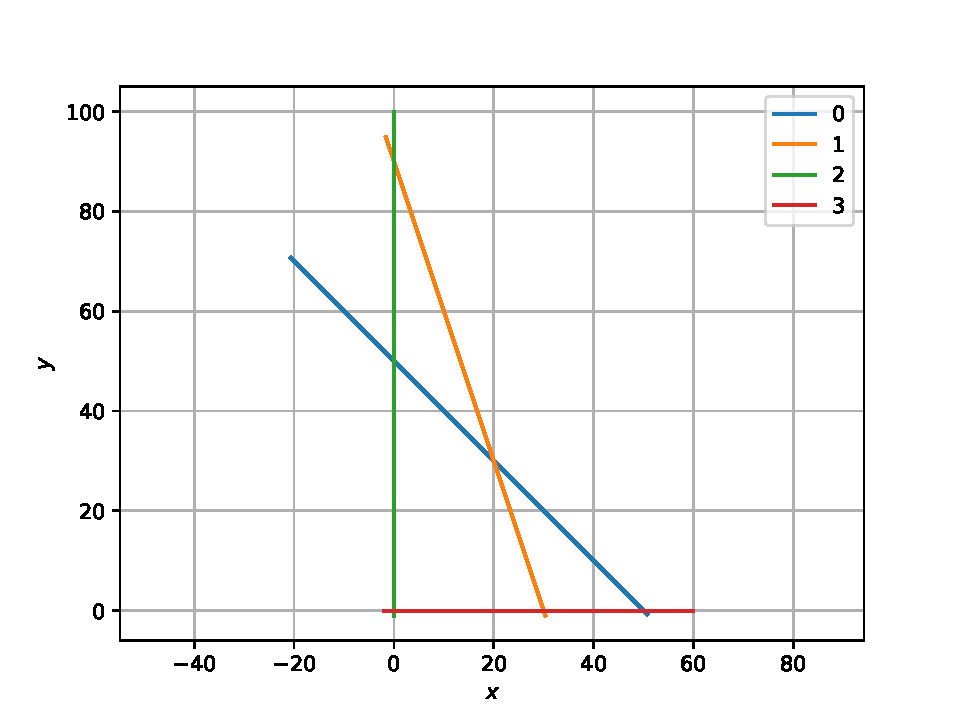
\includegraphics[width=\columnwidth]{./figs/opt/lp_feas_reg.eps}
\caption{}
\label{fig:lp_feas_reg}
\end{figure}

%Verify the solution to graphically.
\item Solve
\begin{align}
\min_{\vec{x}} Z &= \myvec{3 & 9}\vec{x}
\\
s.t. \quad 
\myvec{
1 & 3
\\
-1 & -1
\\
1 & -1
}
\vec{x} &\preceq \myvec{60\\-10\\0}
\\
\vec{x} &\succeq \vec{0}
\label{eq:lp_exam_mult}
\end{align}
\solution The following code
\begin{lstlisting}
codes/opt/lp_cvx_mult.py
\end{lstlisting}
%
is used to obtain
\begin{align}
\vec{x} = \myvec{15\\15}, Z = 180
\end{align}
%
%\item Write a program to plot the constraints for any linear program.

%The region in \eqref{eq:lp_constr} is shown in Fig. \ref{}
\item Solve
\begin{align}
\min_{\vec{x}} Z &= \myvec{-50 & 20}\vec{x}
\\
s.t. \quad 
\myvec{
-2 & 1
\\
-3 & -1
\\
2 & -3
}
\vec{x} &\preceq \myvec{5\\-3\\12}
\\
\vec{x} &\succeq \vec{0}
\end{align}
%
\solution The following code 
\begin{lstlisting}
codes/opt/lp_cvx_nosol.py
\end{lstlisting}
%
shows that the given problem has no solution.
\item Verify all the above solutions using Lagrange multipliers.
\item Repeat the above exercise using the Simplex method.
\item\textbf {(Diet problem)}: A dietician wishes to mix two types of foods in such a
way that vitamin contents of the mixture contain atleast 8 units of vitamin A and 10
units of vitamin C. Food ‘I’ contains 2 units/kg of vitamin A and 1 unit/kg of vitamin C.
Food ‘II’ contains 1 unit/kg of vitamin A and 2 units/kg of vitamin C. It costs
Rs 50 per kg to purchase Food ‘I’ and Rs 70 per kg to purchase Food ‘II’. Formulate
this problem as a linear programming problem to minimise the cost of such a mixture.
\\
\solution Let the mixture contain $x$ kg of food I and $y$ kg of food II.
\\
\begin{table}[!h]
\begin{tabular}{|l|l|l|l|}
\hline
\multirow{2}{*}{Resources} & \multicolumn{2}{l|}{Food} & \multirow{2}{*}{Requirement} \\ \cline{2-3}
                           & I           & II          &                              \\ \hline
Vitamin A                  & 2           & 1           & Atleast 8 Units              \\ \hline
Vitamin C                  & 1           & 2           & Atleast 10 Units             \\ \hline
Cost                       & 50          & 70          &                              \\ \hline
\end{tabular}
\end{table}
%
The given problem can be expressed as
%GOAL: We need to minimize the cost of mixture.\\
%Cost of FOOD I per kg = Rs 50 \\
%Cost of FOOD II per kg = Rs 70 \\
% Minimize $ Z = 50x +70y$\\
% Subject to constraints:\\
% $2x+y>=8$\\
% $x+2y>=10$\\
% $x,y>=0$\\
\begin{align}
\min_{\vec{x}} Z &= \myvec{50 & 70}\vec{x}
\\
s.t. \quad 
\myvec{
2 & 1
\\
1 & 2
%\\
%2 & -3
}
\vec{x} & \succeq \myvec{8\\10}
%\preceq \myvec{5\\-3\\12}
\\
\vec{x} &\succeq \vec{0}
\label{eq:diet}
\end{align}
%
The corner points of the feasible region are available in Table \ref{table:diet_corner_pt} and plotted in Fig. \ref{fig:diet}.
%
\begin{table}[!h]
\begin{tabular}{|l|l|l|l|}
\hline
Corner Point &  $Z=50x+70y$\\
\hline
(0,8)& 560\\
\hline
(2,4)& 380\\
\hline
(10,0)& 500\\
\hline
\end{tabular}
\caption{}
\label{table:diet_corner_pt}
\end{table}
  \begin{figure}[!h]

  \centering
  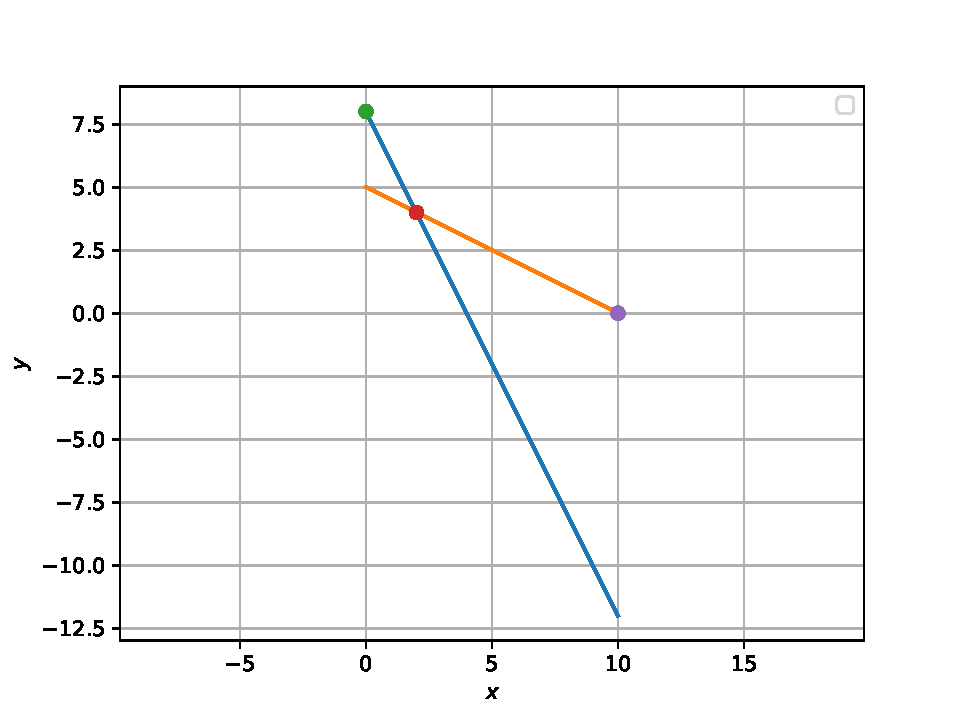
\includegraphics[width=1\linewidth]{./figs/opt/lp_diet.eps}
\caption{}
\label{fig:diet}
  \end{figure}


The smallest value of Z is 380 at the point (2,4). But the feasible region is unbounded therefore we draw the graph of the inequality
\begin{align}
50x +70y<380
\end{align}
to check whether the resulting open half has any point common with the feasible region but on checking it doesn't have any points in common. 
Thus the minimum value of Z is 380 attained at $\myvec{2\\4}$. Hence optimal mixing strategy for the dietician would be to mix 2 Kg of Food I and 4 Kg of Food II.  The following code provides the solution to \eqref{eq:diet}.
%
\begin{lstlisting}
codes/opt/diet.py
\end{lstlisting}



\item \textbf{(Allocation problem)} A cooperative society of farmers has 50 hectare
of land to grow two crops X and Y. The profit from crops X and Y per hectare are
estimated as Rs 10,500 and Rs 9,000 respectively. To control weeds, a liquid herbicide
has to be used for crops X and Y at rates of 20 litres and 10 litres per hectare. Further,
no more than 800 litres of herbicide should be used in order to protect fish and wild life
using a pond which collects drainage from this land. How much land should be allocated
to each crop so as to maximise the total profit of the society?\\
\solution The given problem can be formulated as
\begin{align}
\max_{\vec{x}} Z &= \myvec{10500 & 9000}\vec{x}
\\
s.t. \quad 
\myvec{
20 & 10
}
\vec{x} & \preceq 800
\\
\myvec{
1 & 1
} 
\vec{x} &= 50
\label{eq:allocation}
\end{align}
Fig  \ref{fig:allocation}
shows the intersection of various lines and the optimal point as indicated.
\begin{figure}[h]
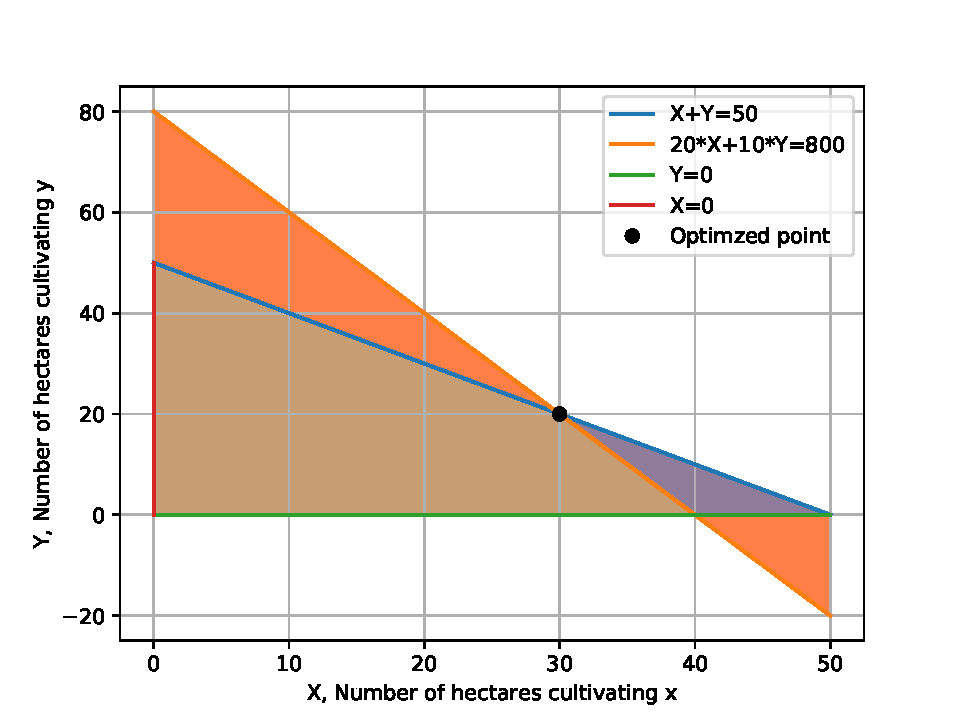
\includegraphics[width=\columnwidth]{./figs/opt/lp_allocation.eps}
\caption{Feasible region for allocation Problem}
\caption{}
\label{fig:allocation}
\end{figure}

The following code provides the solution to \eqref{eq:allocation} at \myvec{30\\20}.
%
\begin{lstlisting}
codes/opt/allocation.py
\end{lstlisting}

\item \textbf{(Manufacturing problem)} A manufacturer has three machines I, II
and III installed in his factory. Machines I and II are capable of being operated for
at most 12 hours whereas machine III must be operated for atleast 5 hours a day. She
produces only two items M and N each requiring the use of all the three machines.
The number of hours required for producing 1 unit of each of M and N on the three
machines are given in Table
	\ref{table:man-prob}
\begin{table}[!h]
	\centering
\begin{tabular}{|c|c|c|c|}
\hline
 \multicolumn{3}{|l}{\textbf{ Number of hours required on machines}}& \\ \cline{2-4}
\hline
\textbf {Items}&\textbf{I}&\textbf{II}&\textbf{III}\\
\hline
M&1&2&1\\
\hline
 N&2&1&1.25\\
 \hline 
\end{tabular}
	\caption{}
	\label{table:man-prob}
\end{table}


She makes a profit of Rs 600 and Rs 400 on items M and N respectively. How many
of each item should she produce so as to maximise her profit assuming that she can sell
all the items that she produced? What will be the maximum profit?
\\
\solution The given problem can be formulated as
\begin{align}
\max_{\vec{x}} Z &= \myvec{80000&12000}\vec{x}
\\
s.t. \quad 
\myvec{
3 & 4
\\
1 & 3
}
\vec{x} & \preceq \myvec{60\\30}
\label{eq:manufacturing}
\end{align}

Fig  \ref{fig:manufacturing}
shows the intersection of various lines and the optimal point as indicated.
\begin{figure}[h]
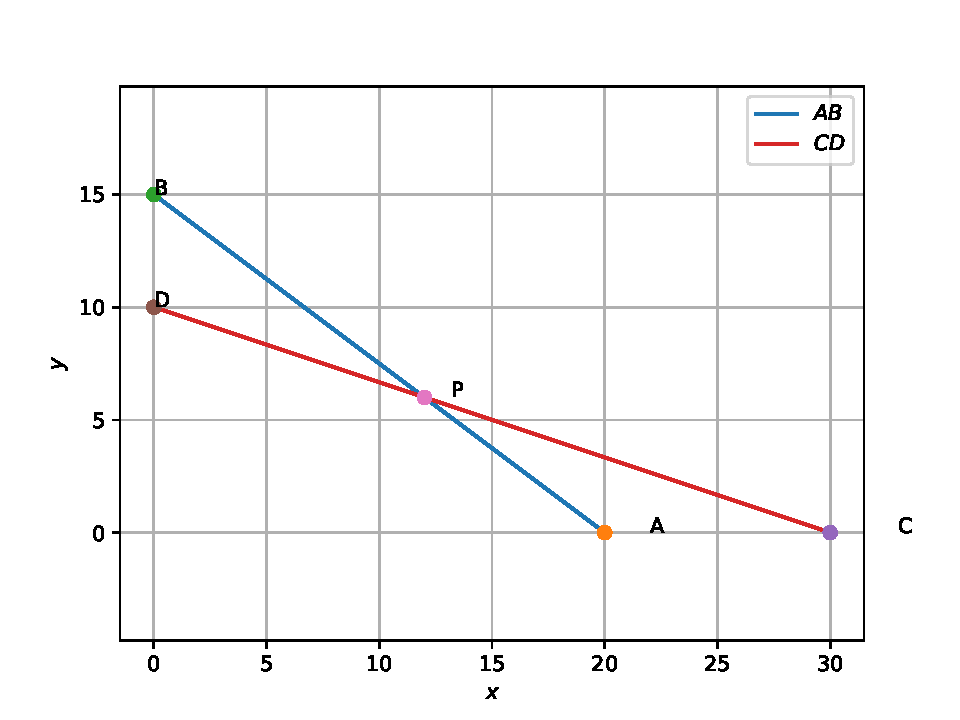
\includegraphics[width=\columnwidth]{./figs/opt/lp_manufacturing.eps}
\caption{Feasible region for manufacturing Problem}
\label{fig:manufacturing}
\end{figure}

The following code provides the solution to \eqref{eq:manufacturing} at \myvec{12\\6}.
%
\begin{lstlisting}
codes/opt/Manufacturing.py
\end{lstlisting}

\item \textbf{(Transportation problem)} There are two factories located one at
place P and the other at place Q. From these locations, a certain commodity is to be
delivered to each of the three depots situated at A, B and C. The weekly requirements
of the depots are respectively 5, 5 and 4 units of the commodity while the production
capacity of the factories at P and Q are respectively 8 and 6 units. The cost of transportation per unit is given below where A,B,C are cost in ruppes:\\
\begin{tabular}{|c|c|c|c|}
\hline
From/To & A & B & C\\
\hline
P & 160 & 100 & 150\\
\hline
Q & 100 &120 & 100\\
\hline
\end{tabular}\\
How many units should be transported from each factory to each depot in order that
the transportation cost is minimum. What will be the minimum transportation cost?
\\
\solution The given problem can be formulated as
\begin{align}
\min_{\vec{x}} Z &= \myvec{10 & -70}\vec{x}
\\
s.t. \quad 
\myvec{
1 & 1
\\
-1 & -1
}
\vec{x} & \preceq \myvec{8\\-4}
\\
\vec{x} &\preceq \myvec{5\\5}
\label{eq:transport}
\end{align}

Fig.  \ref{fig:transport}
shows the intersection of various lines and the optimal point indicated as OPT PT.
\begin{figure}[h]
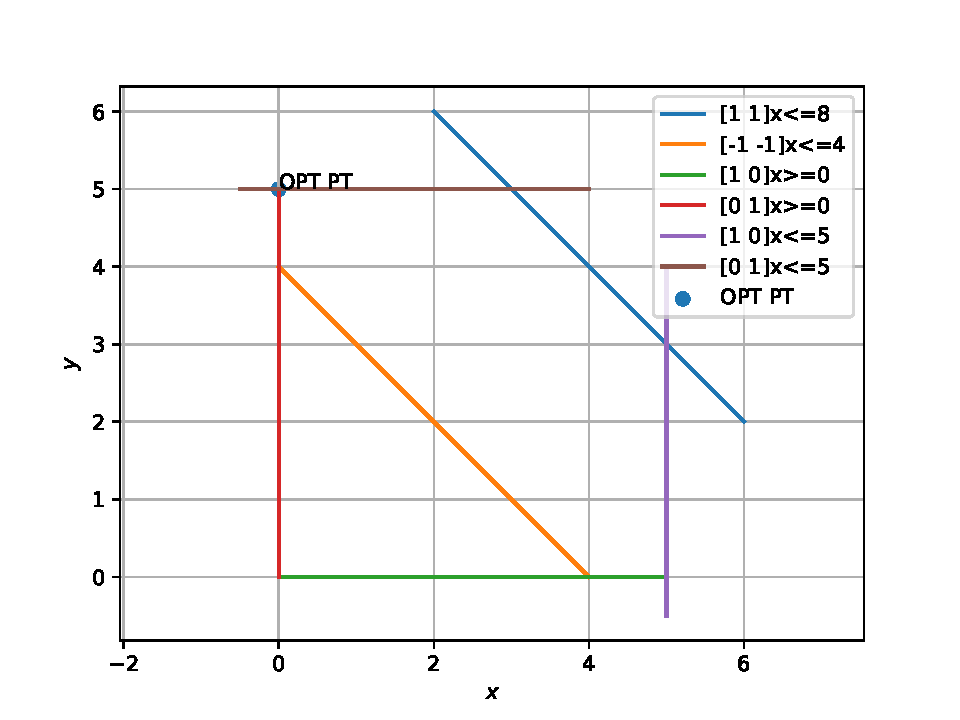
\includegraphics[width=\columnwidth]{./figs/opt/lp_transport.eps}
\caption{Feasible region for Transportation Problem}
\label{fig:transport}
\end{figure}

The following code provides the solution to \eqref{eq:transport} at \myvec{0\\5}.
%
\begin{lstlisting}
codes/opt/Transportation.py
\end{lstlisting}

\end{enumerate}

%\renewcommand{\theequation}{\theenumi}
\end{document}
%
%
